\documentclass[report, a4paper, 12pt]{jsbook}

% しおり機能とコメント機能 (必ず, graphicx系より先に書く事)
\usepackage[dvipdfmx]{hyperref}
\usepackage{pxjahyper}

\usepackage[dvipdfmx]{color}
\usepackage[dvipdfmx]{xcolor}
\usepackage[dvipdfmx]{graphicx}
\usepackage{enumerate}
\usepackage{cover}
\usepackage{abstract}
\usepackage{thesis}
\usepackage{here}
\usepackage{url}
\usepackage[toc,page]{appendix}
\usepackage{tabularx}
\usepackage{multirow}
\usepackage{amsmath}
\usepackage{booktabs}
\usepackage{algorithmic}
\usepackage{algorithm}

% Usage用
%\usepackage{minted}
\usepackage{listings, jlisting}
\lstset{%listings の表示設定
  breaklines = true,%自動で折り返す。
  tabsize = 2,%tabsize
  frame=shadowbox,%枠を上下左右に表示する
  basicstyle = \footnotesize\ttfamily,%\footnotesize,
  keywordstyle=\bfseries\color{green!40!black},
  commentstyle=\itshape\color{purple!40!black},
  lineskip=-0.5zw,
  showstringspaces=false,%文字列中のスペースをちゃんと" "と表示。(デフォルトは文字列中のスペースは可視設定)
  numbers=left,%行番号を左に
  framexleftmargin=6truemm,%行番号をフレーム内に
  numberstyle=\scriptsize,%行番号のサイズ
  stepnumber=1,%1行おきに行番号を
  numbersep=1zw,%ソースと行番号の間隔
  language = C
}%言語設定

\renewcommand{\thelstnumber}{\arabic{lstnumber}:}

\studentid{62008972}
\studentname{佐藤響}
\studentruby{さとうひびき}

%makecover用設定
\covername{佐\ 藤\ \ 響}
\coveryear{令\ 和\ 5\ 年\ 度}
\covertitle{Google PlayストアとXにおける\mbox{}\\ユーザレビューを用いた\mbox{}\\開発者支援ツール}

%makeabstract用設定
\absttitle{Google PlayストアとXにおける\mbox{}\\ユーザレビューを用いた開発者支援ツール}
\abstcontent{%ここに論文要旨を書く. 上寄せなので注意

モバイルアプリのユーザレビューには, そのアプリに関する欠陥の報告やアプリに対する要望など開発者にとって有用な情報が多く存在する. また, Twitterのツイートにはアプリの機能などに関する情報が記述されることが先行研究で示されている. しかし, レビューやツイートの数は膨大であり, 人の手で全て確認するのは不可能に近い. 
先行研究の多くはトピックやカテゴリを事前に定義した上で分類を行うため, ``欠陥の発生している機能ごと''や``アプリに要望している内容ごと''といった粒度の細かい分類はできない. また, アプリごとのレビューの特徴に応じてトピックやカテゴリを変更することはできない. 

本研究では, レビューの中から欠陥の報告やアプリに対する要望といった開発に有用な情報を自動抽出し, 抽出した情報を元にした粒度の細かいクラスタリング手法を提案する. また, その結果を時系列やアプリごとにWebブラウザ上に出力し, 可視化する開発者支援ツールを提案する.
使用するデータは, 過去の論文で収集されたGoogle Playストアのレビュー7,912件とTwitterのツイート1,525,211件に加え, 本研究で新たに収集したGoogle Playストアのレビュー3,967件とTwitterのツイート29,360件である. このデータの中に含まれる開発に有用な情報のみを抽出し, 抽出した情報を活用することで粒度の細かいクラスタリングを可能にした. 
そして, クラスタリング結果をWebブラウザ上で可視化することで, 開発者がレビューを閲覧, 分析しやすくするためのツールを実装した. 

レビューの自動抽出の性能を評価した結果, レビューやツイートの中に開発に有用な情報があるかどうかを判断する精度は高いことが示された. 
しかし, レビューやツイートの中にある有用な情報だけを正確に抽出する精度に関しては, ある程度の高さが示されたものの, 改善の余地があることが確認された. 
クラスタリング性能に関しては, 他の手法と比較した結果, 本手法の精度の高さが確認された. 
そして, 本研究で実装した可視化ツールが開発者にとって有用であることが確認できた. 
}

%maketitle用設定
\title{Google PlayストアとXにおける\mbox{}\\ユーザレビューを用いた開発者支援ツール}
\author{佐藤響}
\date{}

\begin{document}
\makecover    % 表紙ページ生成
\makeabstract % 論文要旨ページ生成
\maketitle    % 内表紙ページ生成
\maketoc      % 目次ページ生成

%\layout

%%%%%%%%%%%%%%%%%%%%%%%%%%%%%%%%%%%%%%%%%%%%%%%%%%%%%%%%%%%%%%%%%%
% 論文本体
% ここに論文の本体のtexファイルを \input{ファイルパス} で入れる. %
% ex. \chapter{テンプレートの使用方法}

この章では, 卒論テンプレートの構成と使用方法について述べる.

\section{設定方法}
thesis.tex を自分のパラメータに変更する.

\section{テンプレートのタイプセット}
この卒論テンプレートから卒論をタイプセットするにあたり, 以下の3つが利用可能である.
\begin{itemize}
\item make
\item omake
\item latexmk
\end{itemize}
以下でそれぞれのコマンドでのタイプセット方法について説明する.

\subsection{make}
% によるタイプセットは以下の利点, 欠点がある.
% \begin{description}
% \item [利点:] 非常に簡単にタイプセットを行える.
% \item [欠点:] makeをインストールしなければならない.
% \end{description}

makeでタイプセットを行う方法をコード\ref{code:make}で示す.
このように端末に打ち込むことで, 卒論本体である thesis.pdf が生成される.
また, 生成された中間ファイルを消去する場合は, コード\ref{code:make-clean}を利用すればよい.

\begin{minipage}{\textwidth}
\begin{lstlisting}[caption={makeコマンド}, label={code:make}, language={sh}]
make
\end{lstlisting}

\begin{lstlisting}[caption={中間ファイルの除去}, label={code:make-clean}, language={sh}]
make clean
\end{lstlisting}

\lstinputlisting[caption={Makefile}, label={code:Makefile}, language={make}]{Makefile}
\end{minipage}

\subsection{omake}
後で書く

\subsection{latexmk}
latexmkはTeXLiveに標準で入っている自動タイプセットツールである.
このツールを利用するには, コード\ref{code:latexmk}を実行すればよい. 
また, latexmkの特徴としてファイルの更新の監視を行い, 更新時に自動でタイプセットを行うことが出来る.
この機能を使用するためには, コード\ref{code:latexmk-pvc}を利用すればよい.

\begin{minipage}{\textwidth}
\begin{lstlisting}[caption={latexmkコマンド}, label={code:latexmk}, language={sh}]
latexmk thesis.tex
\end{lstlisting}

\begin{lstlisting}[caption={latexmkによる自動タイプセット}, label={code:latexmk-pvc}, language={sh}]
latexmk -pvc thesis.tex
\end{lstlisting}

\lstinputlisting[caption={.latexmkrc}, label={code:latexmkrc}, language={perl}]{.latexmkrc}
\end{minipage}                                   %
%%%%%%%%%%%%%%%%%%%%%%%%%%%%%%%%%%%%%%%%%%%%%%%%%%%%%%%%%%%%%%%%%%
\chapter{序論}
\label{chap:jyoron}

%ーーーーーーーーーーーーーーーーーーーーーーーーーーーー
\section{背景}

\subsection{アプリのユーザレビュー}
モバイルアプリのユーザレビュー (以下 : レビュー) とはユーザがそのアプリをインストールして実際に使用した上で, そのアプリに対する評価やコメントをする機能のことである. 
レビューにはユーザがアプリに対して抱いている不満やアプリへの賞賛などが書かれることが多い. また, アプリの欠陥の報告や新しい機能の要望などが記述されることもある. 
アプリの開発者はレビューを参考にしてバグの修正や新しい機能の追加などアプリの品質向上や保守に努めている. 
レビューは配信プラットフォームであるGoogle Playストアや, ソーシャルメディアであるX (旧Twitter)などに書かれることが多い. 

\subsection{Google Playストア}
Google Playストア\cite{google-play-store}とは, Googleが提供しているAndroidやChromeOS向けのデジタルコンテンツ配信サービスである. Google Playストアを使用することにより, アプリやゲームの検索やインストールが可能である. また, 映画や漫画, 書籍の購入やレンタルも可能である. 
Android向けのアプリケーションストアである``Android Market''が2008年に誕生し, 2012年3月6日に``Google Playストア''と改名した. 2022年3月をもって10周年となっており, 現在は数百万以上のコンテンツを配信している\cite{about-google-play}. 
2022年5月時点で190カ国以上の25億人のユーザが毎月Google Playを使用しており, 収益は1,200億ドルに上る\cite{purnima-kochikar}. 

\subsection{X}
X (旧Twitter) \cite{twitter}とは, アメリカのX社が運営しているSNSサービスであり, 2023年7月24日にTwitterから名称が変更されて誕生した. 
このサービスの主な機能は``フォロー'', ``ポスト (旧ツイート) '', ``リポスト (旧リツイート) ''の3つである. 相手のユーザをフォローすることにより相手の投稿を受け取ることができるようになる. ポストとは, 自身の書き込みを投稿することであり, 2022年時点では1日に5億件以上がポストされている\cite{aboutx}. また, 他人のポストをリポストすることにより自分のフォロワーに共有することができる. 
ポストする文章は基本的に全角で140文字, 半角で280文字の制限がある. しかし, 有料の``Twitter Blue''に加入することによって, 全角で2,000文字, 半角で4,000文字までの文章をポストできるようになる. 

アプリの名称がTwitterからXに変わったことに伴い各機能の名称が変更されたため, 本論文では, 各表記を表\ref{tb:twitter}に示すように統一する. 名称がTwitterからXに変更されてからあまり時間が経過していないため, 本論文では一般的に馴染みのある旧名称を使用する. 

\begin{table}[H]
  \caption{本論文での表記}
  \label{tb:twitter}
  \begin{center}
  \begin{tabularx}{\linewidth}{X|X|X}
    \hline
    旧名称&新名称&本論文の表記\\\hline\hline
    Twitter&X&Twitter\\\hline
    ツイート&ポスト&ツイート\\\hline
    リツイート&リポスト&リツイート\\\hline
  \end{tabularx}\end{center}
\end{table}

%ーーーーーーーーーーーーーーーーーーーーーーーーーーーー

\section{本研究の目的}

モバイルアプリのユーザレビューやツイートには, アプリに関する欠陥の報告やアプリに対する要望など開発者にとって有用な情報が多く存在する. しかし, レビューやツイートの数は膨大であり, 開発に有用な情報が埋もれてしまうことがある. 
したがって本研究では, Google PlayストアとTwitterに存在するレビュー, ツイートに含まれる開発に有用な情報を自動で抽出し, 抽出した情報をもとにクラスタリングする手法を提案する. 本研究のクラスタリングは, 事前に定義されたトピックやカテゴリに分類するのではなく, ``欠陥の発生している機能ごと''や``アプリに要望している内容ごと''といった粒度の細かいものとなっている. 
そして, マイニング結果をwebブラウザ上で表示し可視化することにより開発者を支援するツールを提案する. 

%ーーーーーーーーーーーーーーーーーーーーーーーーーーーー

\section{本論文の構成}
本論文の構成は次の通りである. 
\begin{description}

\item[第\ref{chap:kanrenkenkyuu}章 関連研究]\mbox{}\\
本研究の関連研究であるレビューのマイニング, ツイートとレビューの関連性について述べる. \\

\item[第\ref{chap:kibangijyutu}章 基盤技術]\mbox{}\\
本研究で用いる基盤技術である機械学習, BERT, Chinese Whispersについて述べる. \\

\item[第\ref{chap:teian}章 提案]\mbox{}\\
本研究で提案する自動抽出とクラスタリングの手法および可視化ツールについて述べる. \\

\item[第\ref{chap:zisso}章 実装]\mbox{}\\
第\ref{chap:teian}章で提案する手法やツールの実装について述べる. 特にレビューに含まれる開発に有用な情報の自動抽出や抽出結果を元にしたクラスタリング, webブラウザ上で可視化するツールの実装について具体的に述べる. \\

\item[第\ref{chap:kekkahyouka}章 評価]\mbox{}\\
第\ref{chap:zisso}章で実装した手法およびツールの評価実験とその結果について述べる. 3つのResearch Questionをもとに結果を分析し, 考察する. 最後に妥当性の脅威について述べる. \\

\item[第\ref{chap:keturon}章 結論]\mbox{}\\
本研究の結論と研究を行う中で発見された今後の課題について述べる. \\

\end{description}
\chapter{関連研究}
\label{chap:kanrenkenkyuu}




%ーーーーーーーーーーーーーーーーーーーーーーーーーーーー

\section{アプリレビューのマイニング}
近年, テキストをマイニングするための自動化技術 (トピック分類やキーワード抽出など)  をアプリレビューに応用する研究が進んでいる. これらの技術によって, 開発者がアプリレビューを理解・分析するために必要とする労力を軽減することに繋がっている. 
次に示す研究は配信プラットフォームであるGoogle PlayストアやApp Storeから収集されたレビューを対象としている. 
INFAR\cite{infar}はレビューから洞察を発見し, レビューを事前に定義されたトピックに分類したのちに要約を生成する手法である. 定義されるトピックはクラッシュやGUIなどとなっている. 
Wanら\cite{dsa}はアプリレビューの分類の精度を上げるためにフレームセマンティックを用いてアプリレビューに注釈をつけて自動分類するアプローチを提案している. フレームセマンティックとは様々な関係するフレーム要素の状況を記述する概略表現である. この自動分類ではレビューを``Bug report'', ``Feature Request'', ``Others''の3つに分類している. 
また, SUR-Miner\cite{sur-miner}はレビューを表\ref{tb:categories}に示した5つのカテゴリに分類し, 依存関係解析やPart-of-Speechパターンなどの技術を使用して, アプリレビューからいくつかの側面を抽出する. そして最後に概要を可視化する. 
これらの分類における課題として, 事前に定義されたカテゴリやトピックにしか分類することができないため, レビューの特徴に応じてトピックやカテゴリを変更することができない. また, 分類の粒度が粗いことも課題として挙げられる. 

他にも, Casper\cite{caspar}というレビューからアプリの問題に関してユーザが報告したミニストーリー (ユーザアクションと関連するアプリの動作という2種類のイベント)  を抽出し, 合成するための手法が提案されている. 

\begin{table}[H]
  \small
  \caption{Definition of Five Review Categories( \cite{sur-miner} p.763, Table I)}
  \label{tb:categories}
  \begin{center}
    \begin{tabularx}{\linewidth}{l|l|X}
      \hline
      Category&Definition&Examples\\\hline\hline
      Praise&
      \begin{tabular}{l}
        Expressing emotions \\without specific reasons
      \end{tabular}&
      \begin{tabular}{X}
        Excellent!\\I love it!\\Amazing!
      \end{tabular}\\\hline
      Aspect Evaluation&
      \begin{tabular}{l}
        Expressing opinions \\for specific aspects
      \end{tabular}&
      \begin{tabular}{X}
        The UI is convenient.\\I like the prediction text.
      \end{tabular}\\\hline
      Bug Report&
      \begin{tabular}{l}
        Reporting bugs, \\glitches or problems
      \end{tabular}&
      \begin{tabular}{X}
        It always force closes \\when I click the “.com” button.
      \end{tabular}\\\hline
      Feature Request&
      \begin{tabular}{l}
        Suggestions or \\new feature requests
      \end{tabular}&
      \begin{tabular}{X}
        It would be better \\if I could give opinion on it. \\It's a pity it doesn't support \\Chinese.\\I wish there was a “deny” button.
      \end{tabular}\\\hline
      Others&
      \begin{tabular}{l}
        Other categories that \\are defined in 表\ref{tb:categories}
      \end{tabular}&
      \begin{tabular}{X}
        I've been playing \\it for three years
      \end{tabular}\\\hline
    \end{tabularx}
  \end{center}
\end{table}



%ーーーーーーーーーーーーーーーーーーーーーーーーーーーー
\section{ツイートとアプリレビューの関連性}
Deshpandeら\cite{tweetapp}はTwitterからのユーザフィードバックをタイミングと内容の2つの観点から評価し, App Storeのレビューと比較した. 
ツイートとアプリレビューをテキスト分析して, LDA\cite{lda}を用いて分類した. その結果, 426件のツイートと2,383件のレビュー (バグの報告と機能の要求)  のタイミング分析では, 約15\%が最初にTwitterに表示されることが示された. 
また, 15\%のツイートのうち, 72\%はモバイルアプリの機能または動作の側面に関連しているものであった. 一方で, App Storeのレビューはモバイルアプリの機能または動作の側面に関連しているものが全体の80\%であった. 
さらに, 表\ref{tb:topic}に示されているように, ツイートにはアプリに関連する重大な問題や深刻な問題を示すトピックがつぶやかれていることが確認できる. App Storeのトピックもタイミングや回数などの詳細が追加されているものの, 同様の情報を示している. 

\begin{table}[H]
  \caption{Topic analysis from LDA( \cite{tweetapp} p.20, Table IV)}
  \label{tb:topic}
  \begin{center}
    \begin{tabularx}{\linewidth}{|l|l|X|X|}
      \hline
      App&Topic\#&Topics on Twitter&Topics in App Store reviews\\\hline
      Dropbox&
      \begin{tabular}{l}
        1\\2
      \end{tabular}&
      \begin{tabular}{X}
        unable, file, sync, ac- \\cess, try \\connect, fix, mac, open, \\crash
      \end{tabular}&
      \begin{tabular}{X}
        file, upload, unable, \\sync, horrible, time \\crash, every, time, try, \\three
      \end{tabular}\\\hline
      Google cast&
      \begin{tabular}{l}
        1\\2
      \end{tabular}&
      \begin{tabular}{X}
        googlecast, work, bring, \\resolve, session \\reboot, router, tv, add, \\screen
      \end{tabular}&
      \begin{tabular}{X}
        problem, fine, tv, con- \\nect, work \\googlecast, sometimes, \\screen, work, win
      \end{tabular}\\\hline
      LinkedIn&
      \begin{tabular}{l}
        1\\2
      \end{tabular}&
      \begin{tabular}{X}
        wish, meet, announce, \\connect, use \\use, prospects, connect, \\download, wish
      \end{tabular}&
      \begin{tabular}{X}
        option, add, thanks, vi- \\brate, please \\say, make, account, \\launch, fight
      \end{tabular}\\\hline
    \end{tabularx}
  \end{center}
\end{table}
\chapter{基盤技術}
\label{chap:kibangijyutu}


%ーーーーーーーーーーーーーーーーーーーーーーーーーーーー

\section{機械学習}
\subsection{機械学習とは}
機械学習とは, データを分析するための手法の1つであり, 大量のデータをコンピュータが学習し, データに潜んでいるルールやパターンを発見する手法である. コンピュータが自ら学習した成果を用いて未知のデータの予測や発見を可能としており, 反復的に学習させることでデータの中にある規則性, 特徴を発見することができる. 機械学習は現在, 生物学や自動運転, 金融工学などさまざまな分野で大きな影響を与えている. 

機械学習の学習方法には教師あり学習, 教師なし学習, 強化学習の3種類が存在する. 

\subsection{教師あり学習}
読み込んだデータから入力と出力の関係を学習させ, データ間の関係性を学習させる手法である. 学習データには事前に``正解''のラベルを付与される. 
入力された値と正解のラベルのセットを繰り返し学習させることで, 未知の入力された値に対して正解となるデータを予測し, 出力することが可能となっている. 
教師あり学習の具体例には需要予測や株価予測, 画像認識などが挙げられる. 

\subsection{教師なし学習}
教師なし学習とは教師あり学習とは異なり, 学習データに``正解''のラベルは付与せずに, データセットのパターンからデータの関係を認知させる学習手法である. 主に正解と不正解が明確でない問題の解決策として用いられる. 
与えられたデータを繰り返し学習することによりそのデータにどのようなパターンが存在するかをコンピュータ自身が見つけ出すことができる. そのため, 未知のデータに対する予測, 識別を可能とする. 

教師なし学習で行う代表的な例は``クラスタリング''と``次元の削減''である. クラスタリングは複数のデータをそのデータの特徴に応じて幾つかのグループに分けることである. 次元の削減とはデータの次元数を減らすことでデータの特徴を表す情報を抽出することである. 

\subsection{強化学習}
強化学習は, 環境と相互作用しながら報酬をもとに行動を学習する枠組みのことである. 強化学習には方策に従って行動を学習する主体である``エージェント''と状態と報酬をエージェントに返し, エージェントが行動を与える対象である``環境''の2つが存在する. 

強化学習の具体例には将棋や囲碁などのゲームAIやロボットの単純動作の獲得などが挙げられる. Google社のAlphaGoというAIが韓国の囲碁プロ棋士に勝ったことで大きな話題を呼んだ学習方法である. 

%ーーーーーーーーーーーーーーーーーーーーーーーーーーーー

\section{自然言語処理}
自然言語処理 (Natural Language Processing) とは, 人間が使用する言語 (自然言語) をコンピュータが分析する技術である. 自然言語処理によって, 自然言語による大量のテキストデータが持つ意味を解析, 処理することができる. 
自然言語は言葉の曖昧性や意味の重複が含まれている. 例えば, 同じ単語でも文脈が異なると意味が異なることや同じ意味でも様々な表現があることがある. したがって, 意味解釈や文脈解析でコンピュータが人間の意図に反した処理をしてしまうことが課題とされている. 

自然言語処理の活用事例として質問への回答, 文の要約や翻訳, テキスト分類などが挙げられる. 


%ーーーーーーーーーーーーーーーーーーーーーーーーーーーー

\section{BERT}
\subsection{BERTとは}
BERT (Bidirectional Encoder Representations from Transformers) \cite{bert}とは, GoogleのJacob Devlinらによって2018年秋に提案された言語表現モデルである. BERTは, ラベル付けされていないテキストから深い双方向表現を事前学習するように設計されている. その結果, 質問応答や言語推論などの幅広いタスクのためのモデルを作成するために, 出力層を1つ追加するだけで微調整することができる. BERTは11の自然言語処理タスクにおいて, GLUEスコアやSQuAD v1.1による質問応答テストのF1スコアなどで向上が確認された. 

\subsection{学習方法}
BERTは事前学習とファインチューニングの2つのステップからなり, どちらのステップにおいてもtransformerモデルを用いる. transformerとは深層学習のベースとなっているモデルである. RNNやCNNには並列処理ができないという欠点があるが, transformerは再帰や畳み込みは一切行わず, Attentionのみを用いることで並列化を可能にした. 基本的な構成はmulti-head attention層, add\&nom層 (残差結合\&layer normalization) , position-wise FNN層となっている. 

\subsection{事前学習}
事前学習では, Masked Language ModelとNext Sentence Predictionの2つのタスクを解く. Masked Language Modelは入力されたトークンをランダムにマスクし, マスクされたトークンを他のトークンから予測するタスクである. Next Sentence Predictionではある文章に対して, その後に出現する文を並べたペアを正例, ランダムな文章を並べたペアを負例として識別する問題を解く. この問題を解くことにより, 2つの文章が隣り合っているかどうかを予測するよう学習する. 
この2つのタスクは自己教師あり学習である. 自己教師あり学習とは, ラベルが付与されていない大量のデータセットを用いて, プレテキストタスク (擬似的なラベルが自動生成された代わりのタスク) を解くための学習方法である. 自己教師あり学習により人の手作業によるラベル付けを必要とせずに大量のデータで学習することができる. 

\subsection{ファインチューニング}
ファインチューニングでは, ラベル付きデータを用いて特定のタスクに特化するように学習させる. 3.1.1で述べた通り, 解きたいタスクに応じてtransformerの上に出力層を1つ追加する. そしてラベル付きデータを用いて出力層とtransformerのパラメータを更新する. 

%ーーーーーーーーーーーーーーーーーーーーーーーーーーーー

\section{Chinese Whispers}
\subsection{Chinese Whispersとは}
Chinese Whispers (CW) \cite{chinese-whispers}とはグラフクラスタリングのランダム化アルゴリズムである. CWは, 事前にクラスタの数を指定せずに, クラスタの数を自ら選択することができるため, 異なるサイズの分類を扱うことができる. そのため, クラスタの数が事前にわからないNLP問題に適している. 

\subsection{グラフの構築}
まず, ノードとエッジからなる重み付き無向グラフを作成する. これがクラスタリングの対象となるグラフである. ノードはテキスト文書などのデータの要素を表し, エッジはノード間の関連性を表す. 

\subsection{クラスタリングの開始}
クラスタリングの開始時点では, 各ノードはそれぞれ異なるクラスタに属するものとする. すなわち, 1つのノードに対して1つのクラスタが割り振られる. 

\subsection{グラフの反復処理とクラスタの更新}
ノードは少数の反復ステップによってグラフを処理し, 接続されたノードの情報を受け取り, 接続するノードの中で最も近いノードのクラスを継承する. これは現在のノードに対するエッジの重みが最大となるクラスタであるため, 類似したノードが同じクラスタにグループ化される. 最も強いクラスが複数ある場合はランダムで1つ選ばれる. 一方でどのエッジにも接続されていないノードはクラスタリングのプロセスから除外されるため, 一部のノードはクラスタリングされないことがある. 

\subsection{クラスタリングの収束}
グラフの反復処理とクラスタの更新を繰り返すことにより, クラスタが再構築され, 新たなクラスタの構築が進行する. このステップをクラスタリングが収束するまで繰り返した結果, 各ノードは最終的なクラスタに所属する. 
\chapter{提案}
\label{chap:teian}

%ーーーーーーーーーーーーーーーーーーーーーーーーーーーー

\section{概要}
本研究で提案している手法やツールの流れを下記に示す. 

\begin{enumerate}
  \item Google PlayストアとTwitterに投稿されたレビューをスクレイピングして取得, 前処理
  \item レビュー文に含まれる欠陥の報告やアプリに対する要望を示す箇所を自動抽出
  \item 抽出結果を利用しクラスタリング
  \item 分析された結果をwebブラウザ上に可視化
\end{enumerate}

提案手法の流れを図\ref{fig:nagare}に示す. 

\begin{figure}[hbtp]
  \centering
  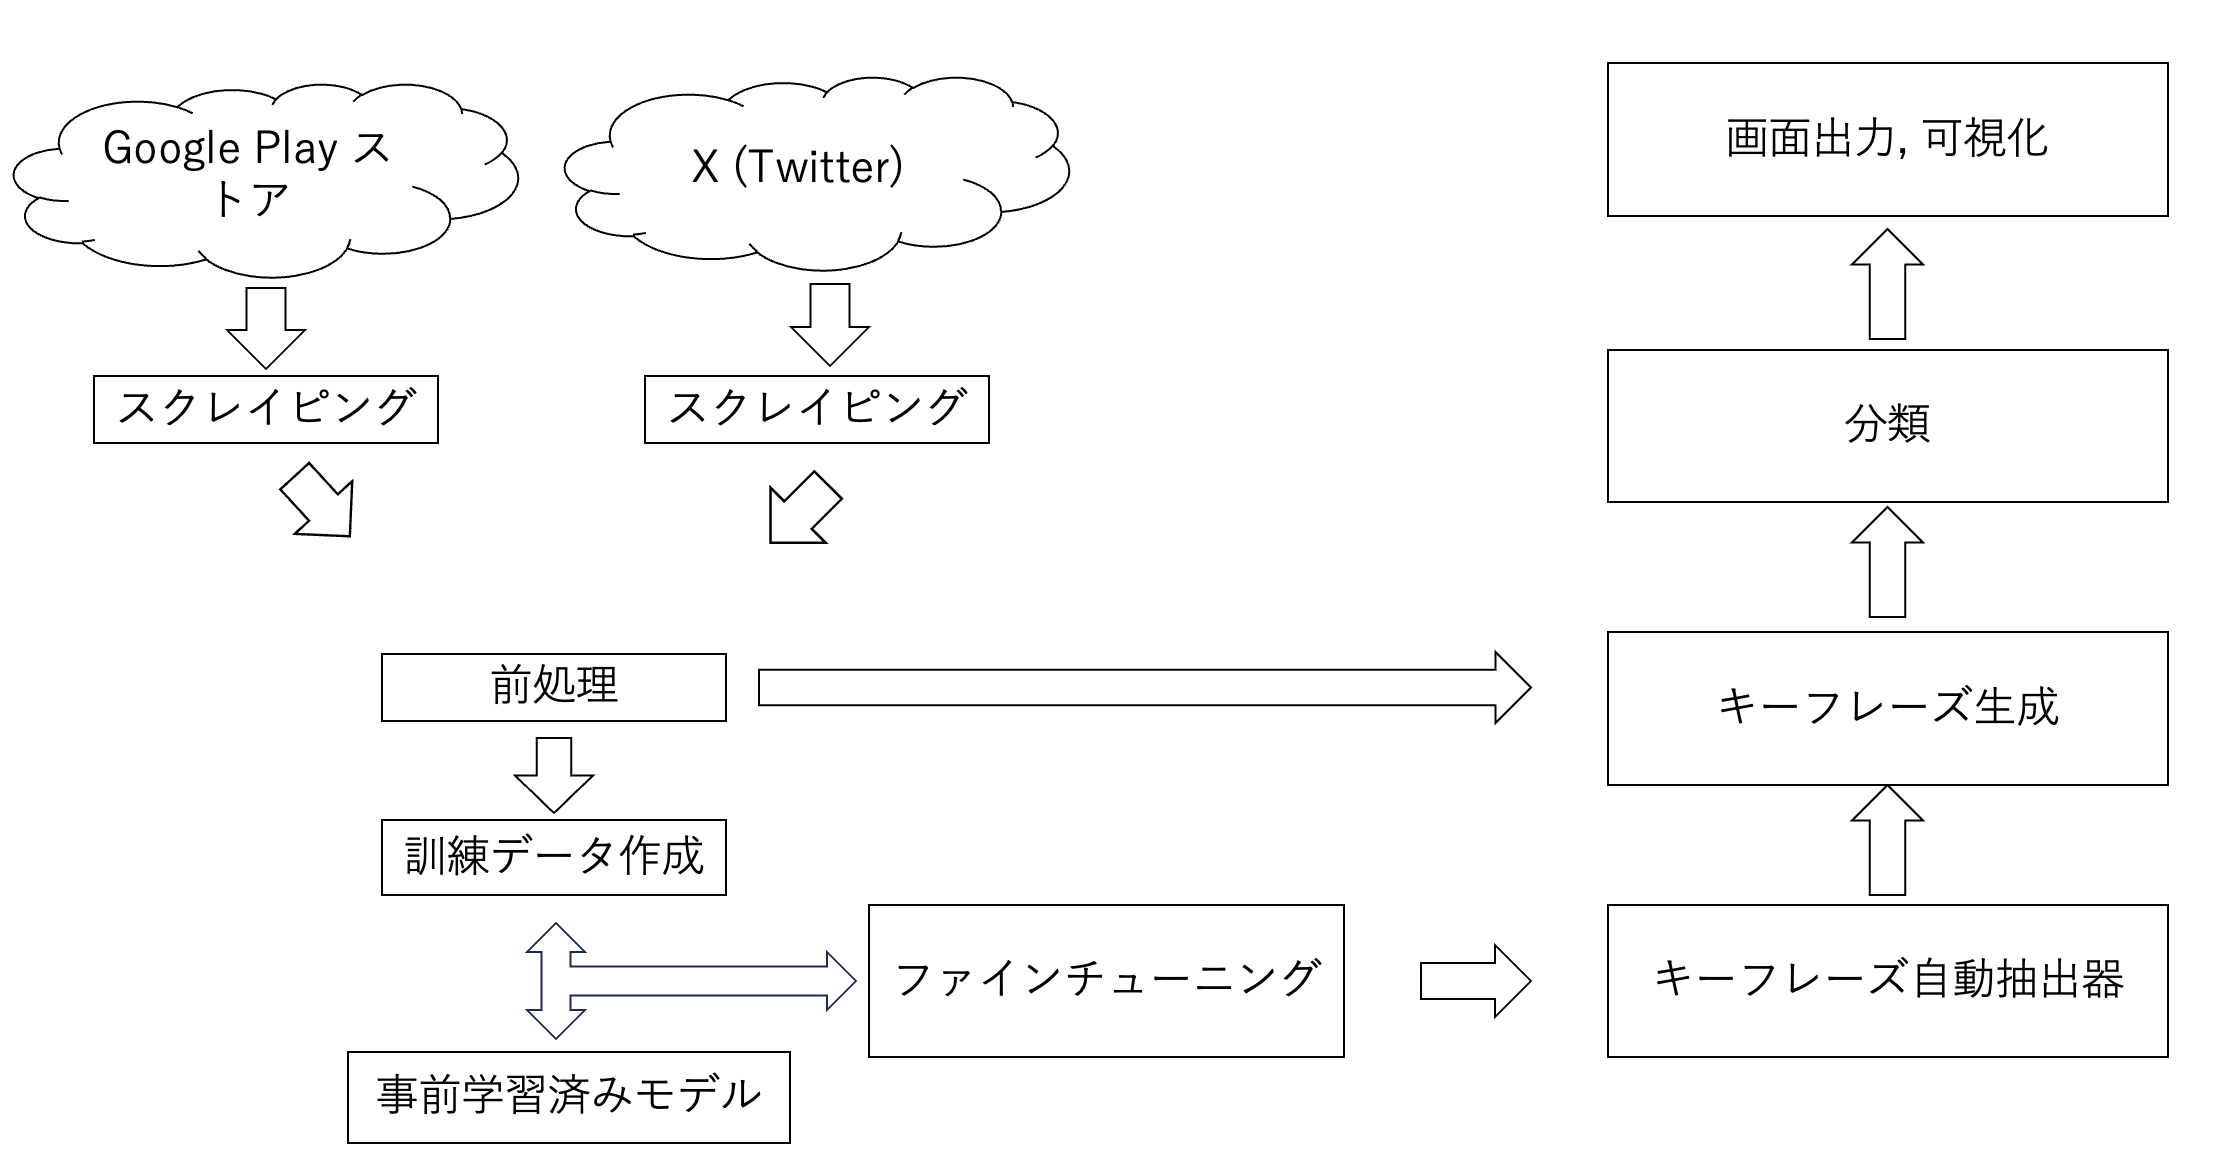
\includegraphics[width=\linewidth]
       {contents/images/zisso_nagare.png}
  \caption{実装した提案手法の流れ\label{fig:nagare}}
\end{figure}

%ーーーーーーーーーーーーーーーーーーーーーーーーーーーー

\section{対象アプリとレビュー}
本研究では川面による先行研究\cite{kawatsura}のデータセットを使用するため対象アプリは先行研究のアプリに合わせている. 注意点として, BuzzVideoは2022年3月をもってサービスを終了しているため, 本研究で収集の対象となるアプリには含まれない. そのため, 本研究で新たに取得するレビューの対象となるアプリはBuzzVideo以外の12のアプリである. 
対象となっているアプリを表\ref{tb:taisyouapuri}に示す. 
\begin{table}[htbp]
  \small
  \caption{本研究の対象アプリ一覧}
  \label{tb:taisyouapuri}
  \begin{center}
  \begin{tabularx}{\linewidth}{l|l|X}
    \hline
    \mbox{アプリ名}\mbox{(一部略称)}&\mbox{Google Playストアの}\mbox{パッケージID}&\mbox{Twitterの}\mbox{検索キーワード}\\\hline\hline
    にゃんトーク&com.akvelon.meowtalk&にゃんトーク\\\hline
    スマートニュース&jp.gocro.smartnews.android&スマートニュース\\\hline
    PayPay&jp.ne.paypay.android.app&paypay\\\hline
    Coke ON&com.coke.cokeon&coke on\\\hline
    Google Fit&com.google.android.apps.fitness&google fit\\\hline
    Simeji&com.adamrocker.android.input.simeji&simeji\\\hline
    Lemon8&com.bd.nproject&lemon8\\\hline
    楽天ペイ&jp.co.rakuten.pay&楽天ペイ\\\hline
    majica&com.donki.majica&majica\\\hline
    LINE MUSIC&jp.linecorp.linemusic.android&line music\\\hline
    BuzzVideo&com.ss.android.article.topbuzzvideo&buzzvideo\\\hline
    ファミペイ&jp.co.family.familymart\verb|_|app&ファミペイ\\\hline
    CapCut&com.lemon.lvoverseas&capcut\\\hline
  \end{tabularx}\end{center}
\end{table}

%ーーーーーーーーーーーーーーーーーーーーーーーーーーーー

\section{事前準備}
本研究で対象としているアプリに関するGoogle PlayストアとTwitterのレビュー及びツイートをスクレイピングし, 分析対象となるデータセットを作成する. 本研究にて使用するデータセットは先行研究によって作成された13個のアプリレビューのデータセットに加え, 本研究で新たに収集した12個のアプリレビューのデータセットを使用する. 
対象アプリを先行研究に合わせた理由としては, 現在, Twitterの利用規約によりツイートの収集可能な数に制限がある影響で, 本研究だけでは十分な数のツイートが収集できなかったためである. Twitterのツイート取得数に関する制限は\ref{sec:x}で詳しく述べる. 
そして, スクレイピングしたデータから有用な箇所を自動抽出するために一般的な自然言語処理で行われる前処理を行う. 

%ーーーーーーーーーーーーーーーーーーーーーーーーーーーー

\section{有用な箇所の自動抽出}
\subsection{概要}
本研究における自動抽出の役割は以下の2つである. 
\begin{itemize}
  \item 前処理された大量のレビューやツイートから開発に有用な文章のみを絞り込む
  \item 文章中からバグの報告やアプリに対する要望に関して記述している部分(以下 : オブジェクト)を抽出する
\end{itemize}
これにより開発に有用な情報のみが取得できる. 

\subsection{使用するモデル}
日本語のデータで事前学習済みの言語表現モデルである日本語BERTに対して質問応答形式のfune-tuningを行うことで自動抽出器を生成する. 
抽出対象となる元の文章の特徴をモデルに理解させるために質問文にその文章がGoogle PlayストアのレビューなのかTwitterのツイートなのかという「カテゴリー」の情報と「アプリ名」という2つの情報を加えることにより学習性能を上げる. 
図\ref{fig:fine-tuning}に質問応答形式によるfine-tuningのモデルを示す. 

\begin{figure}[hbtp]
  \centering
  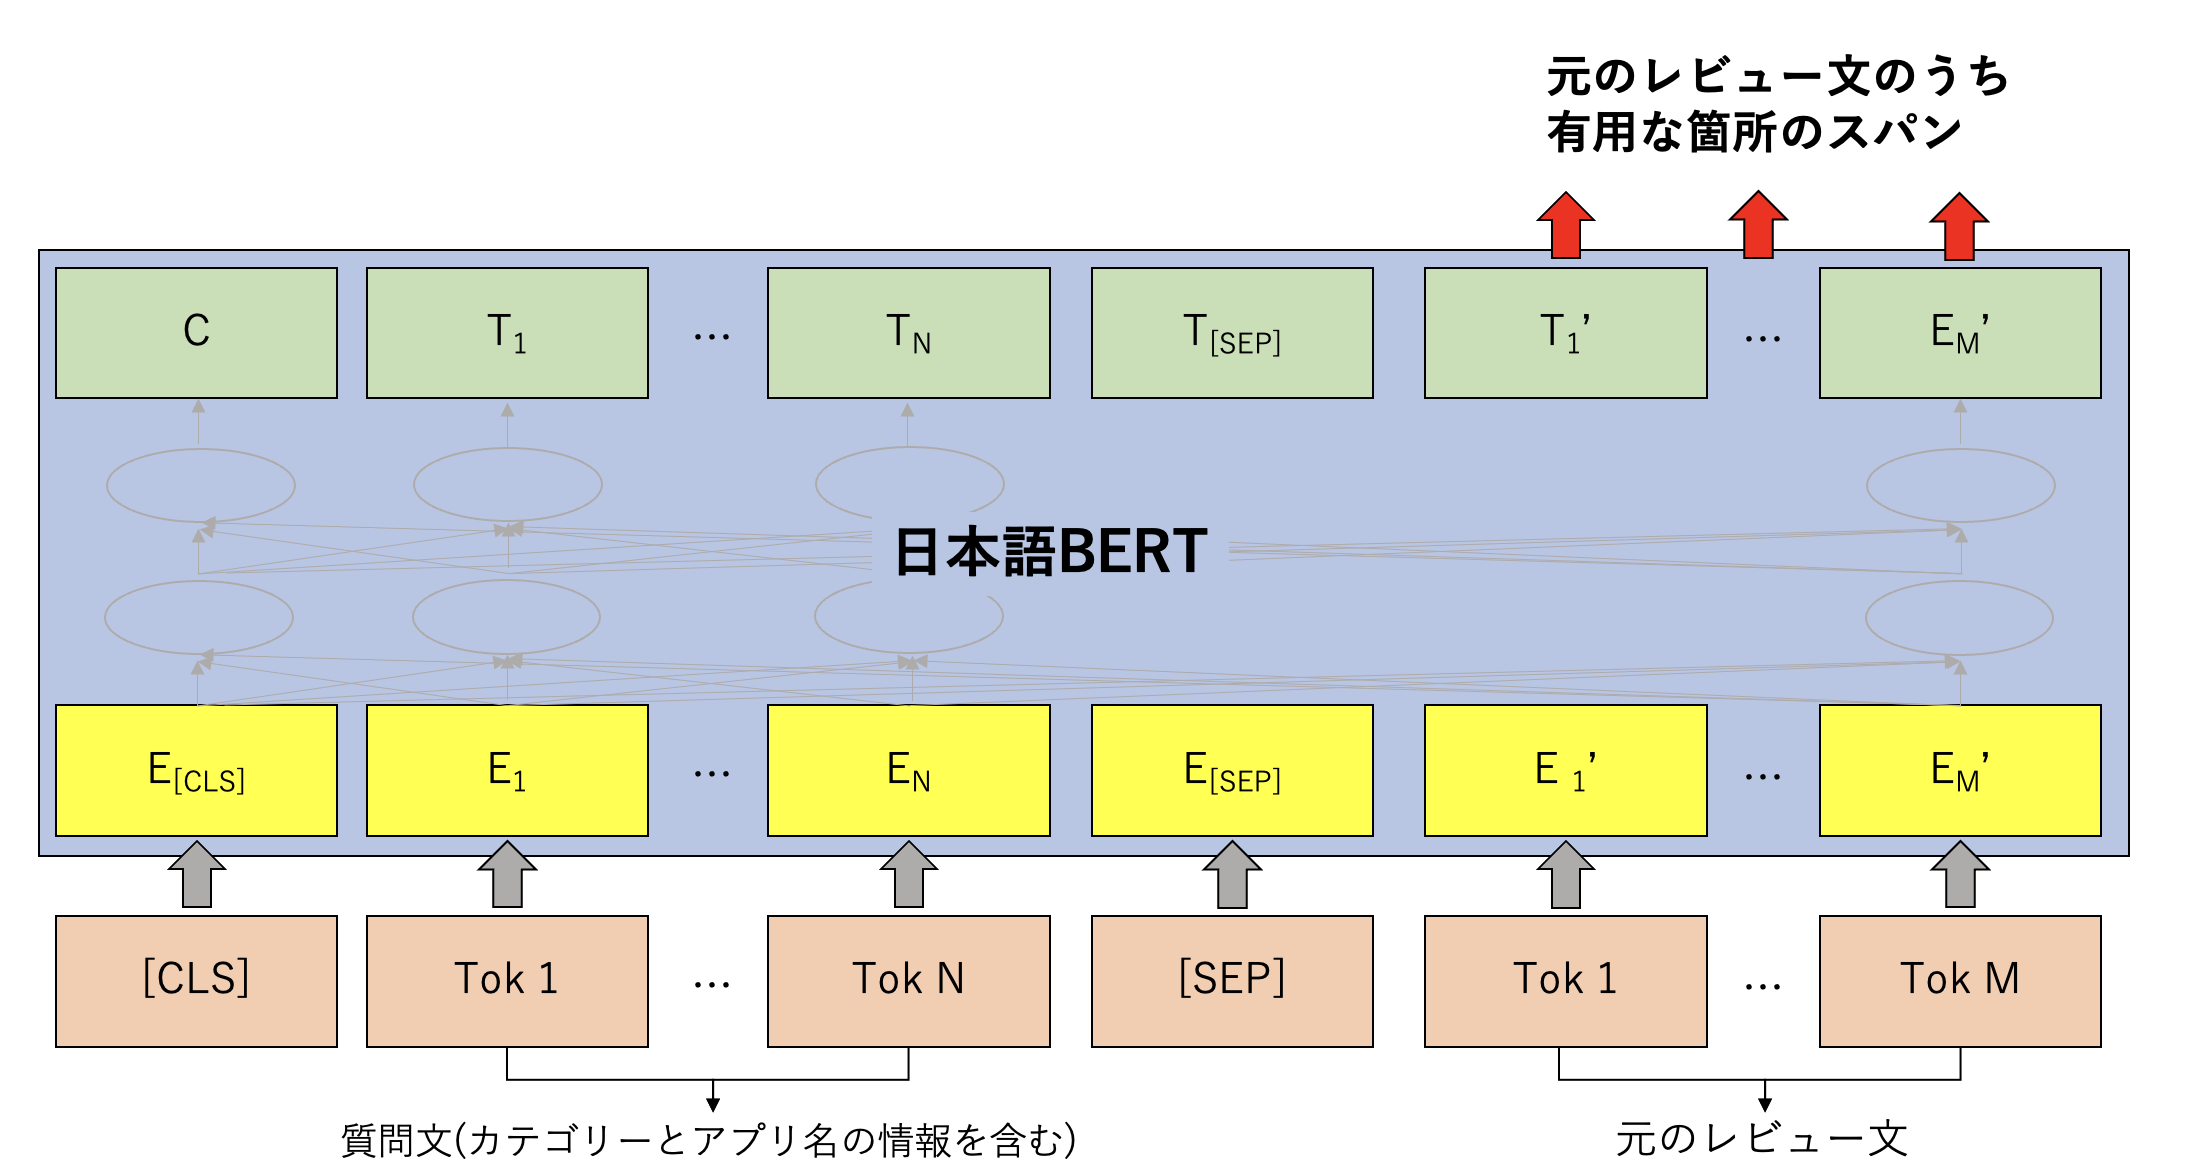
\includegraphics[scale=0.3]
       {contents/images/fine-tuning.png}
  \caption{ファインチューニング\label{fig:fine-tuning}}
\end{figure}

また, 図\ref{fig:answer}に質問文とその答えの例を示す. 質問文にアプリの欠陥やアプリに対する要望を尋ねる文章を与え, その答えとしてオブジェクトを返すようにしている. 

\begin{figure}[hbtp]
  \centering
  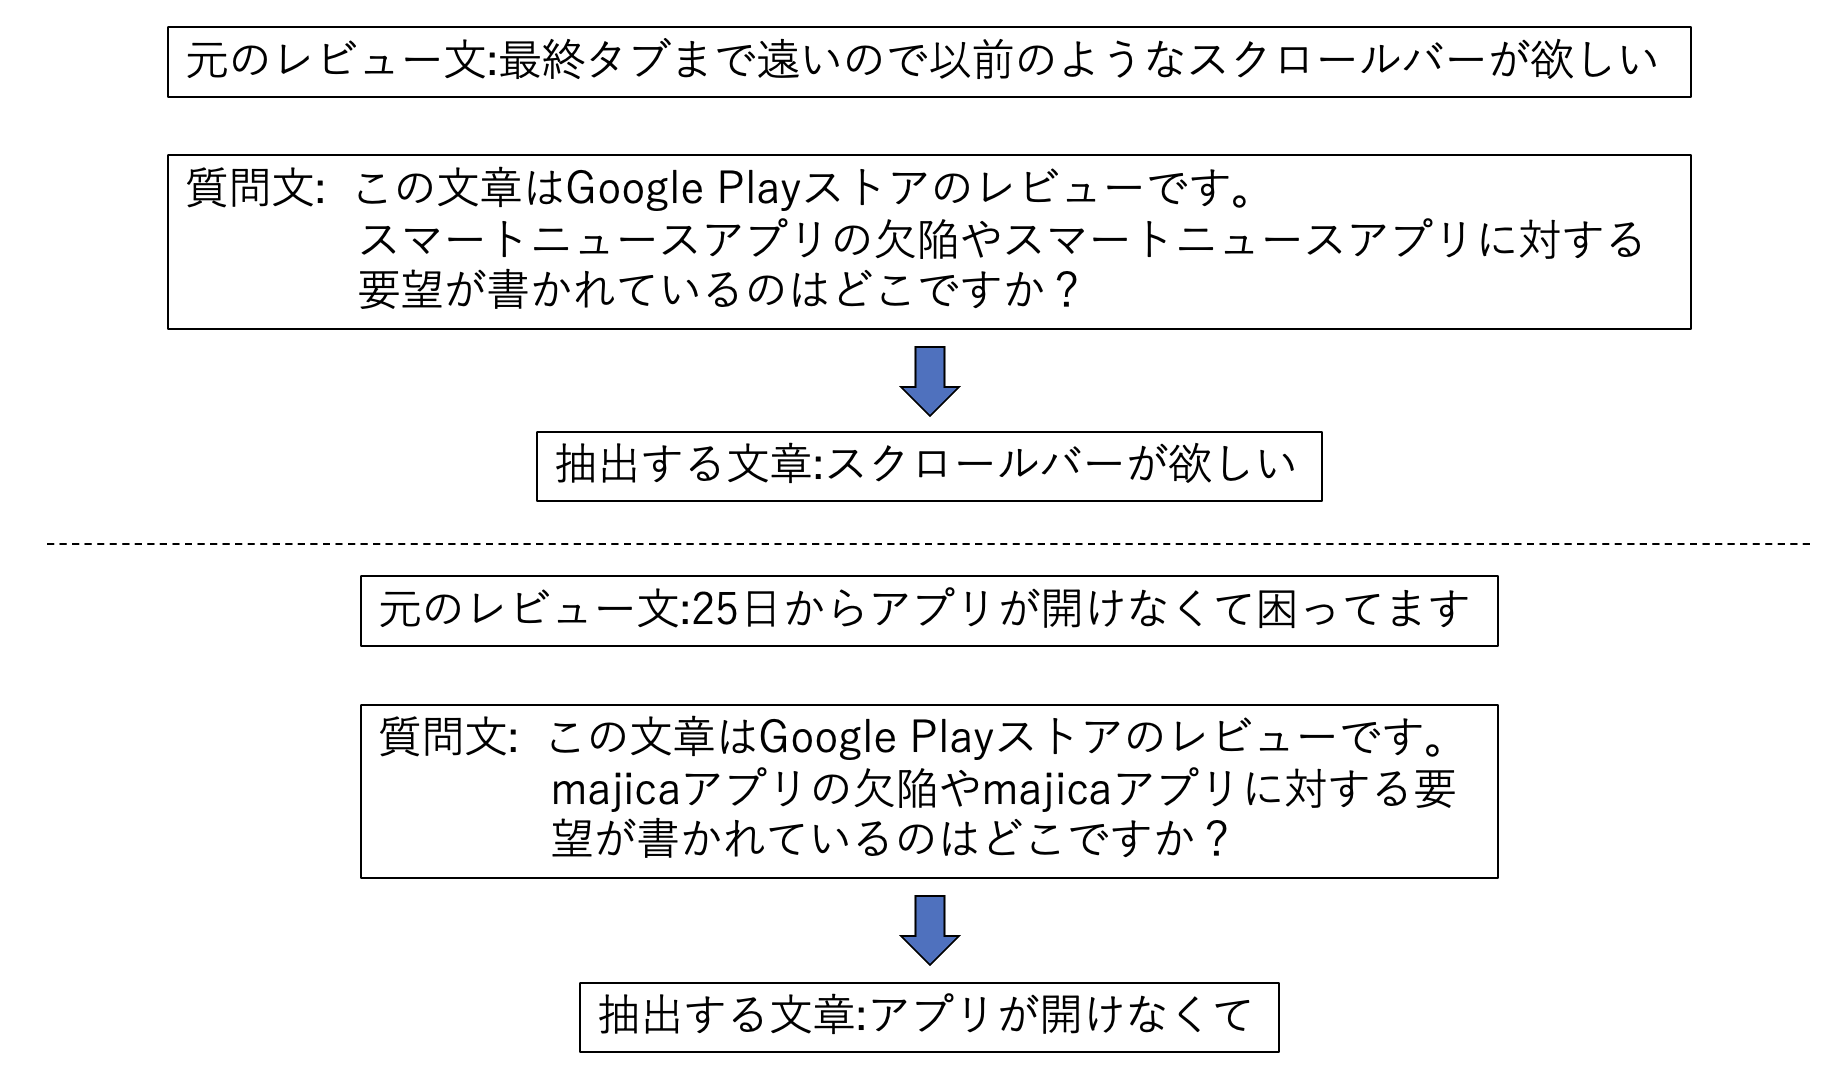
\includegraphics[scale=0.4]
       {contents/images/answer.png}
  \caption{オブジェクトの抽出例\label{fig:answer}}
\end{figure}

%ーーーーーーーーーーーーーーーーーーーーーーーーーーーー

\section{クラスタリング}
\subsection{概要}
本研究におけるクラスタリングの役割は以下の2つである. 
\begin{itemize}
  \item 抽出された各オブジェクトを類似度に応じてクラスタリングする
  \item それぞれのクラスタにおける名称を決める
\end{itemize}

\subsection{クラスタリング手法}
抽出したオブジェクトのクラスタリングにはChinese Whispers\cite{chinese-whispers}を使用したグラフクラスタリング手法を提案する. グラフ作成のために抽出したオブジェクトをSentence-BERTの日本語モデルによってベクトルに変換する. Sentence-BERT\cite{sentence-bert}とは, 事前学習されたBERTモデルとSiamese Networkを使い, 高品質な文ベクトルを作る手法である. このモデルを使用することで, 高品質な文ベクトルが作成できる. 
したがって本研究でのクラスタリング手法は下記の手順である. 
\begin{enumerate}
  \item Sentence-BERTの日本語モデルを用いて, 抽出した文章をベクトルに変換
  \item 重み付き無向グラフを構成し, 抽出したオブジェクトをノードとし, 2つの抽出した文章間のベクトル間のコサイン類似度スコアをノード間の重みとする. スコアがある閾値以上の場合, 2つのノード間にエッジを追加. この閾値は入力ハイパーパラメータであり, 抽出されたオブジェクト間の意味的相関を測定するために使用される. 閾値が高いほどクラスタの結束力が高まる. 
  \item このグラフに対して, Chinese Whispers (CW)を実行し, 問題のある特徴量をクラスタリング
\end{enumerate}

以下の図\ref{fig:clustering}にクラスタリングの概略図を示す. 丸で示されているのが抽出されたオブジェクトを表すノードであり, 点線がエッジである. このエッジは設定された閾値によって変化する. 
\begin{figure}[hbtp]
  \centering
  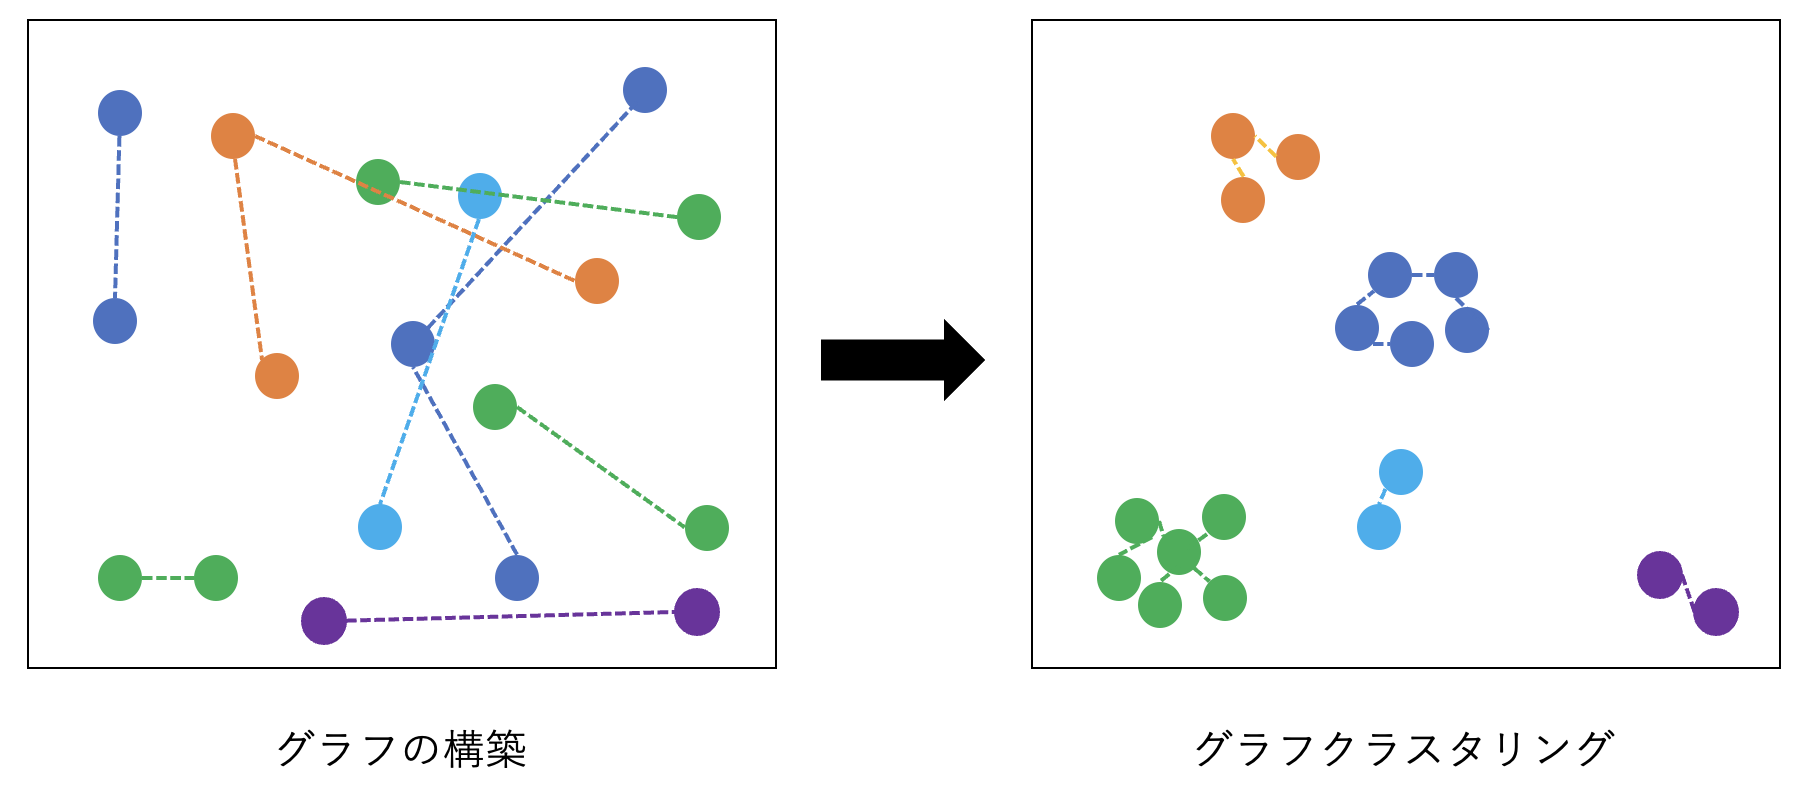
\includegraphics[scale=0.4]
       {contents/images/clustering.png}
  \caption{グラフクラスタリングの概略図\label{fig:clustering}}
\end{figure}

\subsection{各クラスタの名称}
クラスタを作成したら各クラスタの特徴を表す名称を決定する. 
この名称の決定にはKeyBERT\cite{keybert}を使用したキーフレーズの抽出によって実現する. KeyBERTとは, BERTの埋め込みを活用して, 文書に最も類似したキーワードとキーフレーズを作成するキーワード抽出技法である. 
具体的な手順は以下に示す通りである. 

\begin{enumerate}
  \item 文書レベルの表現を得るために, BERTを用いて文書埋め込みを抽出する
  \item N-gramの単語やフレーズについて単語埋め込みを抽出する
  \item コサイン類似度を用いて, 文書に最も類似する単語やフレーズを見つける. 最も類似している単語は, 文書全体を最もよく表現する単語として特定される
\end{enumerate}

%ーーーーーーーーーーーーーーーーーーーーーーーーーーーー

\section{画面出力・可視化}
クラスタリング結果を用いて画面出力し, 可視化を行う. クラスタごとにまとめて表示することで開発者が各レビューを確認しやすいようにする. 
開発者はアプリの修正やアップデートを行った後でユーザがどのようなレビューを挙げているかを特に確認したい. したがって, 特定の機能や期間でのレビュー内容を確認できるよう, レビューが投稿された期間やキーワードで絞り込むことが可能な検索機能を実装した. 
そして, レビューの特徴を確認するために以下2つのグラフを作成した.
\begin{itemize}
  \item 日ごとのレビュー数を表す折れ線グラフ
  \item クラスタに含まれるレビュー数の上位10個を表す棒グラフ
\end{itemize}
この2つのグラフは検索結果に応じて動的に変化するようになっている. 以上の機能をwebアプリとして実装することにより, 開発者がレビューを理解, 分析しやすいように実装されている. 
\chapter{実装}
\label{chap:zisso}

%ーーーーーーーーーーーーーーーーーーーーーーーーーーーー

\section{実装環境}
本研究での実装環境は下記である. 

\begin{itemize}
 \item オペレーティングシステム
    \begin{itemize}
      \item Mac OS Ventura 13.4.1
    \end{itemize}
 \item 実装言語
    \begin{itemize}
      \item Python 3.11.6
    \end{itemize}
\end{itemize}

%ーーーーーーーーーーーーーーーーーーーーーーーーーーーー

\section{Google Playストアのスクレイピング}
本研究で取得するレビュー情報は先行研究に合わせて下記とする. 

\begin{itemize}
 \item reviewId : レビューID
 \item userName : ユーザ名
 \item userImage : ユーザのプロフィール画像
 \item at : 投稿日時
 \item score : 星の数
 \item content : レビュー内容
 \item thumbsUpCount : このレビューが参考になったと評価した人の数
 \item reviewCreatedVersion : レビュー時のバージョン
 \item replyContent : 開発者からの返信の内容
 \item repliedAt : 開発者からの返信日時
\end{itemize}

先行研究では投稿日時が2021年10月21日〜2021年12月15日までの8週間のレビューを収集している. 用意されたGoogle Playストアの各アプリのレビュー数は表\ref{tb:rawreviewnum}の通りである. 
\begin{table}[htbp]
  \caption{収集したGoogle Playストアのレビュー数(\cite{kawatsura} p.16, 表 4.2)}
  \label{tb:rawreviewnum}
  \begin{center}
  \begin{tabular}{l|l}
    \hline
    アプリ名&収集したレビュー数(件)\\\hline\hline
    にゃんトーク&171\\\hline
    スマートニュース&1,651\\\hline
    PayPay&1,052\\\hline
    Coke ON&1,736\\\hline
    Google Fit&372\\\hline
    Simeji&468\\\hline
    Lemon8&72\\\hline
    楽天ペイ&480\\\hline
    majica&706\\\hline
    LINE MUSIC&359\\\hline
    BuzzVideo&375\\\hline
    ファミマのアプリ&290\\\hline
    CapCut&180\\\hline\hline
    合計&7,912
  \end{tabular}\end{center}
\end{table}

この先行研究のデータに加え, 本研究では2023年10月1日~12月15日のレビューを新たに取得する. 新たに取得されたGoogle Playストアの各アプリのレビュー数は表\ref{tb:rawreviewnum2023}の通りである. 
\begin{table}[htbp]
  \caption{収集したGoogle Playストアのレビュー数(2023/10/1〜12/15)}
  \label{tb:rawreviewnum2023}
  \begin{center}
  \begin{tabular}{l|l}
    \hline
    アプリ名&収集したレビュー数(件)\\\hline\hline
    にゃんトーク&\\\hline
    スマートニュース&\\\hline
    PayPay&\\\hline
    Coke ON&\\\hline
    Google Fit&\\\hline
    Simeji&\\\hline
    Lemon8&\\\hline
    楽天ペイ&\\\hline
    majica&\\\hline
    LINE MUSIC&\\\hline
    ファミマのアプリ&\\\hline
    CapCut&\\\hline\hline
    合計&
  \end{tabular}\end{center}
\end{table}

Google PlayストアのレビューをスクレイピングするためにPythonのプログラムである(\verb|get_google_play_review.py|)を作成した. このプログラムの作成にあたり, Pythonのライブラリであるgoogle-play-scraperを使用する. google-play-scraperでは外部依存関係なしでPython用のGoogle Playストアを簡単にクロールするためのAPIが提供されている\cite{google-play-scraper}. 
このライブラリを使用することにより, アプリのパッケージ名, 言語, 取得する数, 順序を指定してレビューの一覧を取得することができる. 

%ーーーーーーーーーーーーーーーーーーーーーーーーーーーー

\section{Xのスクレイピング}
\label{sec:x}
本研究で取得するツイート情報は先行研究に合わせて下記とする. 
\begin{itemize}
 \item id : ツイートID
 \item content : ツイート内容
 \item at : ツイート日時
\end{itemize}

まず, 先行研究で収集したツイート数を表\ref{tb:rawtweetnum}に示す. 

\begin{table}[htbp]
  \caption{収集したTwitterのツイート数(\cite{kawatsura} p.18, 表 4.3)}
  \label{tb:rawtweetnum}
  \begin{center}
  \begin{tabular}{l|l}
    \hline
    アプリ名&収集したツイート数(件)\\\hline\hline
    にゃんトーク&2,525\\\hline
    スマートニュース&50,590\\\hline
    PayPay&880,319\\\hline
    Coke ON&84,424\\\hline
    Google Fit&13,496\\\hline
    Simeji&205,327\\\hline
    Lemon8&4,376\\\hline
    楽天ペイ&11,111\\\hline
    majica&3,649\\\hline
    LINE MUSIC&184,873\\\hline
    BuzzVideo&41,656\\\hline
    ファミマのアプリ&8,867\\\hline
    CapCut&33,998\\\hline\hline
    合計&1,525,211
  \end{tabular}\end{center}
\end{table}

この先行研究に加え, 本研究では新たに2023年10月1日~12月15日のポストを取得する. Xのポスト取得に関してはTwitter APIを使用してスクレイピングを行う. Twitter APIのプランに関してはFree, Basic, Pro, Enterpriseの4つのプランが用意されておりそれぞれ料金や使用できる機能などが異なる. 大規模なサービスやビジネス向けのEnterpriseプラン以外の3つのプランの違いの一部を表\ref{tb:xplan}に示す. 
表\ref{tb:xplan}よりポストを取得するためにはBasicプラン以上に加入する必要がある. Basicプランに加入した場合でも合計で30,000件しか取得されないため本研究では先行研究のデータセットを追加で使用することとした. Xの利用規約によると, Xが提供するインターフェイスを介して行うスクレイピング以外は禁止としている. そのため, seleniumなどを使用したスクレイピングは断念し, 過去の論文のデータを使用することとした. 

\begin{table}[htbp]
  \caption{プランとできること}
  \label{tb:xplan}
  \begin{center}
  \begin{tabular}{|l|c|c|c|}
    \hline
    &Free&Basic&Pro \\\hline\hline
    料金&無料&月額100ドル&月額5,000ドル \\\hline
    月間ポスト数の上限&1,500&3,000&300,000 \\\hline
    月間ポスト取得数&0&10,000&1,000,000 \\\hline
  \end{tabular}\end{center}
\end{table}

Twitter APIを使用してポストを取得するためにPythonのプログラムである(\verb|get_tweet.py|)を作成した. このプログラムではTwitter APIにアクセスするためのライブラリであるTweepy\cite{tweepy}を使用した. まずAPIキーなどの4つの認証情報をセットする. 次にClientクラスのsearch\_resent\_tweetメソッドを使用してツイートを取得する. 
このメソッドは最大過去7日間まで遡ってツイートを取得できる. search\_all\_tweetsメソッドでは全てのツイートを取得できるが, ``Academic Research''という学術用の用途でAPI承認されたユーザーしか使用できないため本研究では使用しなかった. 
先行研究と同じ情報を取得するために, 本研究では引数として以下のものを与えた. 
\begin{itemize}
 \item max\_resul : 検索結果の最大数. 10〜100の数値で, デフォルトは10
 \item query: 検索ワード
 \item tweet\_field: ツイートフィールドを選択. 今回はツイート日時を取得するために["created\_at"]とした. 
 \item end\_time: 期間の終わりを指定できる(UTCタイムスタンプ)
\end{itemize}

新たに取得したXのポスト数を表\ref{tb:rawtweetnum2023}に示す

\begin{table}[htbp]
  \caption{収集したXのポスト数}
  \label{tb:rawtweetnum2023}
  \begin{center}
  \begin{tabular}{l|l}
    \hline
    アプリ名&収集したツイート数(件)\\\hline\hline
    にゃんトーク&\\\hline
    スマートニュース&\\\hline
    PayPay&\\\hline
    Coke ON&\\\hline
    Google Fit&\\\hline
    Simeji&\\\hline
    Lemon8&\\\hline
    楽天ペイ&\\\hline
    majica&\\\hline
    LINE MUSIC&\\\hline
    ファミマのアプリ&\\\hline
    CapCut&\\\hline\hline
    合計&
  \end{tabular}\end{center}
\end{table}

%ーーーーーーーーーーーーーーーーーーーーーーーーーーーー

\section{前処理}
機械学習によるレビューに含まれる有用な箇所の自動抽出の精度を上げるために, GooglePlayストアとXから取得したデータに対して前処理を行うプログラム(\verb|preprocessing_google.py|, \verb|preprocessing_twitter.py|)を作成した. この処理では以下に示す処理を行う. この処理は一般的な自然言語処理の手法を参考としている. 
\begin{itemize}
  \item 英語を全て小文字に揃える. 
  \item 以下の文字列を削除. 
    \begin{itemize}
      \item 「」【】()()『』
      \item @@から始まるメンション
      \item \#から始まるタグ
      \item URL
      \item 半角空白,全角空白
      \item 絵文字
      \item 日本語を含まないレビュー
    \end{itemize}
  \item レビューやツイートには, 異なるバグの報告や新しい機能の要望に関する文が2文以上からなるものがある. そのため, 「。」「.」「!」「!」「?」「!」「\verb|\n|」「\verb|\r\n|」でそれぞれの文に分割する. 
\end{itemize}
以下の図\ref{chap:preprocessing}がレビューを前処理した例である. 2つの文で構成されているため「。」で区切り分割している. また絵文字は削除されている. 

\begin{figure}[hbtp]
 \centering
 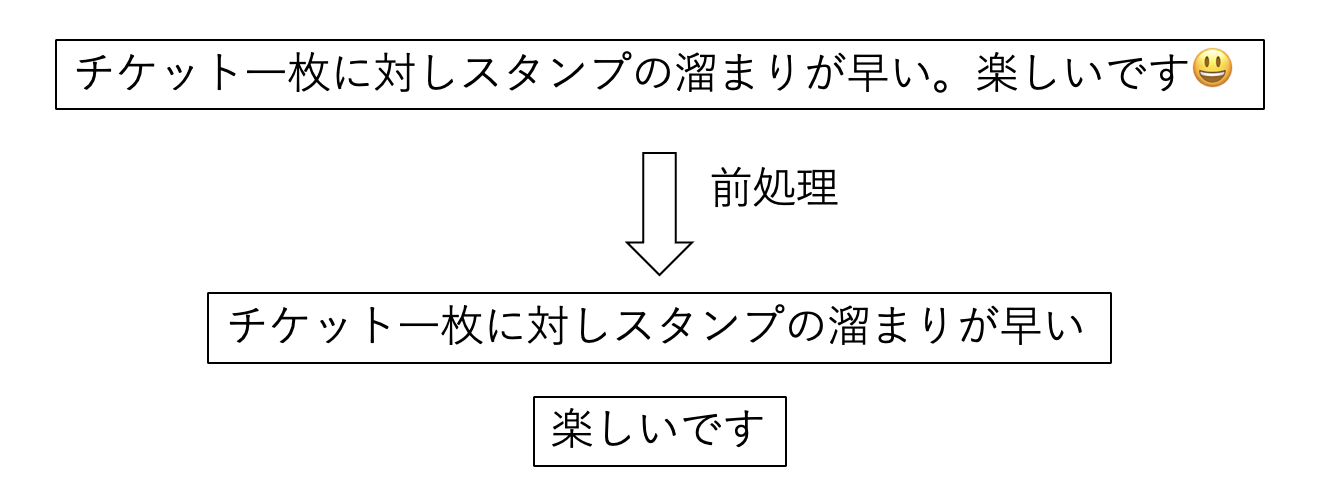
\includegraphics[scale=0.5]
      {contents/images/preprocessing.png}
 \caption{前処理の例\label{chap:preprocessing}}
\end{figure}

前処理した結果をcsvファイルにて保存する. 保存する項目としては, 投稿日時(at), レビューのid(reviewId)またはツイートid(id), そして, 前処理した文章である. 図\ref{tb:googlecsv}, 図\ref{tb:twittercsv}に前処理結果後のcsvファイルの一部を示す. 

\begin{table}[htbp]
  \caption{Google Playストアレビューの前処理結果(buzzvideo)}
  \label{tb:googlecsv}
  \begin{center}
  \begin{tabularx}{\linewidth}{|l|l|X|}
    \hline
    at&reviewId&content\\\hline\hline
    2021-12-15 19:25:30&gp:AOqpTOHj6w ...&バズビデオを見て、感動をありがとう\\\hline
    2021-12-15 12:28:09&gp:AOqpTOHleV ...&内容が残酷で異常な人が多い\\\hline
    2021-12-15 11:09:50&gp:AOqpTOHG7O ...&分かりづらい\\\hline
    2021-12-14 15:16:33&gp:AOqpTOGWvT ...&ばず29さいって人が投稿してる動画すべて虚偽動画なのでアカウント削除と動画削除して欲しい\\\hline
    2021-12-14 15:16:33&gp:AOqpTOGWvT ...&あるだけで大迷惑です\\\hline
    2021-12-14 15:16:33&gp:AOqpTOGWvT ...&二度と登録し直せないよう個体識別番号で縛ってください\\\hline
    2021-12-14 15:16:33&gp:AOqpTOGWvT ...&お願いします\\\hline
  \end{tabularx}\end{center}
\end{table}

\begin{table}[htbp]
  \caption{ツイートの前処理結果(BuzzVideo)}
  \label{tb:twittercsv}
  \begin{center}
  \begin{tabularx}{\linewidth}{|l|l|X|}
    \hline
    at&id&content\\\hline\hline
    2021-12-15T23:55:11.000Z&1471267626655825922&芸能人に似てる気がするけど名前が思い出せない\\\hline
    2021-12-15T23:53:43.000Z&1471267256659509249&驚愕男性が豆乳を飲むべき3つの理由\\\hline
    2021-12-15T23:53:43.000Z&1471267256659509249&男だからこそ注目したい豆乳のメリットとは\\\hline
    2021-12-15T23:53:17.000Z&1471267149746679813&感情を乗せた歌声と歌詞に聞き惚れちゃう♪壊れかけのradio\\\hline
    2021-12-15T23:53:10.000Z&1471267120264904705&kkと眞子の酷い嘘\\\hline
    2021-12-15T23:53:10.000Z&1471267120264904705&恐ろしい真実が明らかに\\\hline
  \end{tabularx}\end{center}
\end{table}

%ーーーーーーーーーーーーーーーーーーーーーーーーーーーー

\section{有用な箇所の自動抽出}
\subsection{データセット}
モデルのfine-tuningに使用されるデータセットとして, Google PlayストアとXのツイートからそれぞれ5,000件ずつ合計で10,000件のデータをランダムに抽出し手作業で有用な箇所を抽出した. データセットの作成は情報工学科の学部4年生2人がそれぞれ手作業で行い, お互いの抽出した箇所が異なっていたものは議論することにより決定した. 
データセットには前処理したデータを利用したcsvファイルを使用する. このcsvファイルにはid,アプリ名,投稿日時,本文, 手動で抽出した結果の5つの情報が入っている. idは前処理したデータを識別するために与えられ, Google Playストアのレビュー文はg\_{index}, twitterのツイートのidはt\_{index}とする. 
10,000件のデータセットのうち, 6,000件を訓練データ, 2,000件を検証用データ, 2,000件をテストデータとする. 質問応答形式のfine-tuningを行うために, csv形式であるデータセットをソースコード\ref{json}に示すようにjson形式に変換する. 

\begin{lstlisting}[caption=データセット.json,label=json]
  {
    "version": "v2.0", 
    "data": [
      {
        "title": "モバイルアプリのレビュー", 
        "paragraphs": [
          {
            "context": "本アカウントのフォローやリツイートお願いします",
            "qas": [
              {
                "id": "t_2223388",
                "question": "この文はTwitterのツイートです。
                             paypayアプリの欠陥やpaypayアプリに対する
                             要望が書かれているのはどこですか?",
                "is_impossible": true,
                "plausible_answers": [{"text": "", "answer_start": -1}],
                "answers": [{"text": "", "answer_start": -1}]
              }
            ]
          },
          {
            "context": "11/25前後からアプリを開いても強制終了、
                      会員バーコードもクーポンも何も出せない状態、
                      これでは買い物ができないと、こちらのレビュー
                      を見に来て沢山の方が同じ状態であることが
                      わかった",
            "qas": [
              {
                "id": "g_6041", 
                "question": "この文章はGooglePlayストアのレビューです。
                            majicaアプリの欠陥やmajicaアプリに対する
                            要望が書かれているのはどこですか?",
                "answers": [{"text": "アプリを開いても強制終了、
                                      会員バーコードもクーポン
                                      も何も出せない", 
                             "answer_start": -1}], 
                "is_impossible": false
              }
            ]
          }, ...
        ]
      }
    ]
  } 
\end{lstlisting}

このjsonファイルは下記の構成になっている. 
\begin{itemize}
  \item version: バージョンを表す. 今回は答えられない質問を含むSQuAD 2.0と同じバージョンのため, v2.0とする
  \item title: contextのタイトル
  \item paragraphs: context1つとそれに関連する質問, 答えがリスト形式で保持されている
  \item qas: 質問と回答がリスト形式となっている
  \item context: 元の文章(抽出する前の文章)
  \item id: 設定したid
  \item question: 質問文
  \item is\_impossible: 答えられない質問ならtrue, それ以外はfalse
  \item plausible\_answers: 質問が答えられない時のみ存在し, 問題文から答えになりうる部分を抽出
  \item answers: contextから抜き出した答えとその位置情報がリスト形式で保持されている. 答えを複数用意することもできる. 
  \item text: contextから抜き出した答えのテキスト情報(抽出する文章)
  \item answe\_start: contextから抜き出した答えの位置情報
\end{itemize}

\subsection{モデルのfine-tuning}
用意したデータセットを用いて事前学習済みモデルをfine-tuningする. 本研究では事前学習済みモデルとしてHuging FaceのTransformersを通して利用できる東北大学のモデル\cite{tohoku}を使用する. このモデルは日本語のWikipediaのデータを用いて学習されている\cite{tohoku}. 
この東北大学が公開している日本語BERTのうち, whole word maskingを適用して学習させているモデル\cite{masking}を用いる. whole word maskingとは事前学習時に単語ごとでマスクするかどうかを決め, マスクする単語に対応するサブワードを全てマスクする方式である. モデルのパラメータは以下に示す通りである. 
\begin{itemize}
  \item 学習率: 3e-5
  \item エポック数: 10
  \item バッチサイズ: 12
\end{itemize}

実装にはTransformersに含まれるスクリプトであるrun\_squad.pyを用いる. 

\subsection{自動抽出}
fine-tuningを行ったモデルを使用して自動抽出を行う. 前処理したGooglePlayストアのデータ14,051件と, twitterのデータ4,634,319件のデータから有用な箇所を自動抽出する. 

結果は表\ref{tb:googleqa}に示すようにcsv形式で保存する. 

\begin{table}[htbp]
  \caption{Google Playストアレビューの自動抽出結果(google\_fit)}
  \label{tb:googleqa}
  \small
  \begin{center}
  \begin{tabularx}{\linewidth}{|l|l|X|X|X|}
    \hline
    id&app\_name&datetime&context&prediction\\\hline\hline
    g\_955&coke\_on&2021-11-27 11:17:03&商品が出ない事が何回か発生しました&商品が出ない\\\hline
    g\_956&coke\_on&2021-11-02 12:15:37&使用している端末が、利用できる端末の一覧表にないため、サポートは期待できない&使用している端末が、利用できる端末の一覧表にない\\\hline
    g\_959&coke\_on&2021-11-11 15:32:50&そもそも自販機側が黄色点滅していなくて買えないことが多過ぎです&自販機側が黄色点滅していなくて買えない\\\hline
    g\_961&coke\_on&2021-11-14 23:13:26&今まではcoke\_on対応を優先してかっていたが、これからはコカコーラ製品全般をできるだけ買わないようにする&今まではcoke\_on対応を優先してかっていたが、これからはコカコーラ製品全般をできるだけ買わないようにする\\\hline
    g\_964&coke\_on&2021-10-24 12:30:07&自販機との接続を早くしてほしい&自販機との接続を早くしてほしい\\\hline
    g\_965&coke\_on&2021-11-11 16:43:39&やっと繋がっても先にキャンペーン広告が出てすぐに買えないのが不親切&キャンペーン広告が出てすぐに買えない\\\hline
    g\_969&coke\_on&2021-12-07 08:28:27&コークオンパスのフリー20プランの残り回数が分かりやすく表示してほしい&コークオンパスのフリー20プランの残り回数が分かりやすく表示してほしい\\\hline
    g\_973&coke\_on&2021-11-23 14:51:45&反応しない&反応しない\\\hline
    g\_977&coke\_on&2021-11-11 18:22:04&2本以上の購入はとても使えません&2本以上の購入はとても使えません\\\hline
    g\_978&coke\_on&2021-11-01 11:06:09&それと対応自販機との連携が悪い&自販機との連携が悪い\\\hline
    g\_980&coke\_on&2021-10-22 03:22:06&動きが遅い&動きが遅い\\\hline
    g\_982&coke\_on&2021-11-22 11:58:45&ただ自分のスマホのストレージが小さく、データ容量が大きいため今回一先ず削除いたします&自分のスマホのストレージが小さく、データ容量が大きい\\\hline
  \end{tabularx}\end{center}
\end{table}

%ーーーーーーーーーーーーーーーーーーーーーーーーーーーー

\section{クラスタリング}
抽出した文章をその文章が示す意味に応じてクラスタリングする. クラスタリングするために日本語Sentence-BERTクラスを定義する. ソースコード\ref{sentence-bert}に日本語Sentence-bertクラスを示す. 
\_mean\_pooling関数でモデルの出力とAttention Maskを用いて, 文の埋め込みを生成するための平均プーリングを行い, encode関数で文のリストから各文章の埋め込みを求める. 
すなわち, 日本語のBERT用に転移学習したBERTを用いて各トークンの埋め込みを求め, 平均を取ることにより文全体の埋め込みを求めている. 

\begin{lstlisting}[caption=clustering.py,label=sentence-bert]
  class SentenceBertJapanese:
    def __init__(self, model_name_or_path, device=None):
        self.tokenizer = BertJapaneseTokenizer.from_pretrained(model_name_or_path)
        self.model = BertModel.from_pretrained(model_name_or_path)
        self.model.eval()

        if device is None:
            device = "cuda" if torch.cuda.is_available() else "cpu"
        self.device = torch.device(device)
        self.model.to(device)

    def _mean_pooling(self, model_output, attention_mask):
        token_embeddings = model_output[0] #First element of model_output contains all token embeddings
        input_mask_expanded = attention_mask.unsqueeze(-1).expand(token_embeddings.size()).float()
        return torch.sum(token_embeddings * input_mask_expanded, 1) / torch.clamp(input_mask_expanded.sum(1), min=1e-9)

    @torch.no_grad()
    def encode(self, sentences, batch_size=8):
        all_embeddings = []
        iterator = range(0, len(sentences), batch_size)
        for batch_idx in iterator:
            batch = sentences[batch_idx:batch_idx + batch_size]

            encoded_input = self.tokenizer.batch_encode_plus(batch, padding="longest", 
                                           truncation=True, return_tensors="pt").to(self.device)
            model_output = self.model(**encoded_input)
            sentence_embeddings = self._mean_pooling(model_output, encoded_input["attention_mask"]).to('cpu')

            all_embeddings.extend(sentence_embeddings)

        # return torch.stack(all_embeddings).numpy()
        return torch.stack(all_embeddings)
\end{lstlisting}

ソースコード\ref{model}に示されるようにSentenceBertJapaneseクラスを用いて, 引数に日本語モデル名を与えることによりインスタンスが生成され, モデルの読み込みが完了する. このモデルを使用して抽出された文章をベクトルに変換する. 

\begin{lstlisting}[caption=clustering.py,label=model]
  model = SentenceBertJapanese("sonoisa/sentence-bert-base-ja-mean-tokens")
\end{lstlisting}

次に, それぞれの抽出した文章をノード, ノードのベクトル間のコサイン類似度をエッジとする無向グラフを作成する. 作成されたグラフからChinese Whispersによりクラスタリングが実行される. 
クラスタリングした結果, それぞれの文章にクラスタの番号(以下 : クラスタ番号)が振られ, クラスタ番号が同じものが同じクラスタとなり番号が近いものは意味的相関が近いことを表す. コサイン類似度の閾値を決めることによりどの程度の類似文を同じクラスタと定義するのかが決定される. 本研究では検証を重ねた結果, 閾値は0.8とした. 
結果はcsvファイルに保存される. 表\ref{tb:clustering}に示されるように抽出した文章にクラスタ番号が振られる. 

\begin{table}[htbp]
  \caption{抽出した文章とクラスタ番号(google\_fit)}
  \label{tb:clustering}
  \begin{center}
  \begin{tabularx}{\linewidth}{|X|c|}
    \hline
    prediction&cluster\\\hline\hline
    十分歩いて108歩とかふざけんな&273\\\hline
    278歩に減っていた&274\\\hline
    再起動しても直らない&275\\\hline
    接続/連携を適宜確認しておく必要がある&276\\\hline
    歩いた歩数より足りない&279\\\hline
    使えない&280\\\hline
    使えない&280\\\hline
    歩けない&280\\\hline
    使えない&280\\\hline
    動かなかった&280\\\hline
    反応しない&280\\\hline
    使い方も分からない&280\\\hline
    使えない&280\\\hline
    使えない&280\\\hline
    動かなくなった&280\\\hline
    長期放置されてるんでしょうか&281\\\hline
    下がるって何故でしょうか&282\\\hline
    カウントされなくなる&283\\\hline
    何もカウントしなくなった&283\\\hline
    カウント出来ていない&283\\\hline
    カウントされず&283\\\hline
    記録ができませんと&283\\\hline
    計測しなくなった&283\\\hline
    カウントされなくなった&283\\\hline
    カウントしない&283\\\hline
    全くカウントされていない&283\\\hline
    カウントしなくなりました&283\\\hline
    データが反映されなくなった&283\\\hline
  \end{tabularx}\end{center}
\end{table}


%ーーーーーーーーーーーーーーーーーーーーーーーーーーーー

\section{画面出力・可視化}
\subsection{実装環境}
webアプリケーションの実装に使用した言語, フレームワークは以下となっている. 
\begin{itemize}
    \item フロントエンド: HTML/CSS, JavaScript
    \item バックエンド: Python
    \item フレームワーク: Flask
\end{itemize}

\subsection{概要}
分類した結果の含まれたcsvファイルの情報をバックエンド側で処理し, リストを作成する. そのリストをフロントエンド側に渡し処理することでレビューの情報をwebブラウザ上に表示することができる. 

\subsection{画面構成}
画面は大きく分けて一覧画面とアプリごとの詳細画面の2つである. 

一覧画面では全てのアプリに対する日ごとのレビュー数を表す折れ線グラフを表示する. 
このグラフをGoogle Playストアのレビューとツイートの2つ作成する. 

アプリごとの詳細画面では, アコーディオンメニューを使用して抽出した文章の一覧をクラスタごとに表示する. また, 抽出した文章をクリックすると投稿日時や元のレビュー文がモーダルウィンドウで表示する. 
そして, 日ごとのレビュー数を表す折れ線グラフとクラスタに含まれるレビュー数の上位10個を表す棒グラフの2つのグラフを表示する. 

\subsection{検索のロジック}
検索項目である期間とキーワードを指定するとその情報がバックエンド側に渡され, 処理することでリストを更新する. 更新されたリストの情報をフロント側に渡すことで検索結果が反映される. 
ツイートのリストを検索結果に応じて更新するソースコード\ref{search}を示す. 

\begin{lstlisting}[caption=view.py, label=search]
  path = f'../クラスタリング/twitter_{app_name}.csv'
  is_file = os.path.isfile(path)
  if is_file:
      with open(path, 'r', encoding='utf-8-sig') as twitter_csv_file:
          twitter_csv_reader = csv.reader(twitter_csv_file)
          twitter_rows = list(twitter_csv_reader)
          twitter_rows = sorted(twitter_rows, reverse=False, key=lambda x: x[2]) # 日付で並び替え
  # 検索結果のリスト作成
  search_result = []
  for row in twitter_rows:
      if start_date <= row[2][:10] <= end_date:
          if keyword != '':
              if keyword in row[3]:
                  search_result.append(row)
          else:
              search_result.append(row)
  twitter_rows = search_result
\end{lstlisting}

\subsection{グラフの作成}
グラフの作成にはplotly.js\cite{plotly}を用いる. plotly.sjとはグラフ生成ライブラリであり, 3Dグラフや統計グラフなど40を超えるグラフタイプが同梱されている\cite{plotly}.
plotly.jsで作成されたグラフにはオプションとしてズーム機能やグラフのダウンロード機能が付随している. 
日付ごとのレビュー数に関するグラフを表示するソースコード\ref{graph}を示す. 設定したタグをDOMのターゲットにしてplotly.jsに書き換えてもらう. graphsはバックエンド側で作成された日付とその日のレビュー数に関する二次元リストであり, 横軸に日付, 縦軸にレビュー数を取るグラフである. 
dataのtypeでグラフタイプを指定でき, layoutでタイトルや表の大きさを指定できる. 

\begin{lstlisting}[caption=detail.html, label=graph]
  <div class="graph-title">日付ごとのレビュー数の推移</div>
  <div id="scatter"></div>

  <script>
      // 横軸: 日付
      var labels = JSON.parse('{{ graphs | map(attribute=0) | list | tojson | safe }}');
      // ラベル用日付
      var displayLabels = [];
      for (var i = 0; i < labels.length; i += 5) {
          displayLabels.push(labels[i]);
      }
      var values = JSON.parse('{{ graphs | map(attribute=1) | list | tojson | safe }}');

      var data = [{
          x: labels,
          y: values,
          type: 'scatter',
      }];

      var layout = {
          title: '日付ごとのレビュー数の推移',
          height: 600,
          width: 1200,
          xaxis: {
              tickvals: displayLabels,  // 配列の5つおきの目盛り位置を指定
          }
      };

      Plotly.newPlot('scatter', data, layout);
  </script>
\end{lstlisting}



\chapter{評価}
\label{chap:kekkahyouka}

\section{概要}
本論文の提案手法について評価するために, 次に示すの3つのRQを用意した. 

\begin{itemize}
  \item RQ1: レビューの抽出性能はどの程度か
  \item RQ2: クラスタリングの性能はどの程度か
  \item RQ3: 可視化ツールの有用性はどうか
\end{itemize}

RQ1では, BERTを用いた抽出モデルによるレビューの自動抽出性能について評価した. 評価する際は, モデルがレビューにキーフレーズがあるかどうかを正確に判断できるか, キーフレーズがある場合, そのキーフレーズを正確に抽出できるかという2点についてそれぞれ評価する. 

RQ2では, まず, 本研究のクラスタリング手法として使用したChinese Wispersで作成されるグラフの適切な閾値について検証した. そして, Chinese Whispersのクラスタリング性能を, K-Meansと階層型クラスタリングという2つのクラスタリング手法と比較して評価した. 

RQ3では, 本論文で実装した可視化ツールが開発者にとって有用なものあるかどうかを評価した. 一般的にレビューの閲覧や確認で使用されるGoogle Playストアのレビュー欄と比較することで, 本ツールの有用性を示す. 

\section{RQ1:レビューの抽出性能はどの程度か}
\subsection{評価方法}\label{method}
作成された抽出モデルの抽出性能について調査する. 使用するデータセットは\ref{dataset}項で記述したデータセット10,000件のうち, テストデータとした2,000件である. このテストデータに対して自動抽出を行い, 手動で抽出した結果と自動抽出した結果を比較した. 
この自動抽出に関しては, レビューにキーフレーズがないものは答えのない文章と判断し, レビューにキーフレーズがある場合は答えのある文章と判断する. また, 答えのある文章に関してはレビューにある有用な情報を答えとする. 
答えがある問題では, 次に示す3つの場合に分けて評価する. 

\begin{itemize}
  \item 抽出したキーフレーズが完全に一致している場合
  \item 抽出したキーフレーズが部分的に一致している場合
  \item 抽出したキーフレーズが全く一致していない場合
\end{itemize}

\subsection{結果}
\ref{method}の評価方法に基づいて検証された結果を表\ref{tb:qa}に示す. 

\begin{table}[H]
  \caption{抽出結果}
  \small
  \label{tb:qa}
  \begin{center}
  \begin{tabularx}{\linewidth}{X|r}
    \hline
    答えがある問題数&468\\\hline
    答えがある問題の正当数&261\\\hline
    答えがある問題の部分一致正答数&124\\\hline
    答えがない問題数&1532\\\hline
    答えがない問題の正答数&1483\\\hline\hline
    答えがある問題の正答率&55.8\%\\\hline
    答えがある問題の部分一致を含めた正答率&82.3\%\\\hline
    答えがない問題の正答率&96.8\%\\\hline\hline
    全体の正答率&87.2\%\\\hline
    部分一致を含めた全体の正答率&93.4\%\\\hline
  \end{tabularx}\end{center}
\end{table}

答えがない問題の正答率は96.8\%と非常に精度の高い結果となった. すなわち, 本研究で作成された抽出モデルはレビューにキーフレーズがあるかどうかを判別する精度が高いことが示された. 
一方で, 答えがある問題の正答率は55.8\%とあまり精度が高くないものの, 部分一致を含めた正答率は82.1\%と比較的高い結果が得られた. 

\subsection{考察}
正答率が下がってしまった原因に関して考察する. 
答えがある問題, すなわちキーフレーズが存在する文章のうち誤って抽出してしまった例を表\ref{tb:mistake}に示す.

\begin{table}[H]
  \caption{誤答となったテスト結果 (答えあり) }
  \small
  \label{tb:mistake}
  \begin{center}
  \begin{tabularx}{\linewidth}{X|X|X}
    \hline
    元の文章&自動抽出した回答&手動抽出した回答\\\hline\hline
    店で使えずに仕方なく現金で払いました&&店で使えず\\\hline
    とにかく地図検索がクソ&とにかく地図検索がクソ&地図検索がクソ\\\hline
    急に曲が止まって何しても流れないから端末再起動させたらようやく流れた&急に曲が止まって何しても流れないから端末再起動させたらようやく流れた&急に曲が止まって何しても流れない\\\hline
    データのカウント数が減ることがある&データのカウント数が減る&カウント数が減ることがある\\\hline
    ウォーキングで設定してるのに10分の1しかカウントしない&ウォーキングで設定してるのに10分の1しかカウントしない&10分の1しかカウントしない\\\hline
    類似アプリと比べて突出した利点もなく、あえてlinemusicを選ぶ理由がない&&類似アプリと比べて突出した利点もなく\\\hline
    コークオンを使おうとしてるのに、使えないなんでか、解らない&コークオンを使おうとしてるのに、使えないなんでか&コークオンを使おうとしてるのに、使えない\\\hline
    12月1日正午再び開けなくなりバーコードのみ表示&再び開けなくなりバーコードのみ表示&開けなくなりバーコードのみ表示\\\hline
    クレジットカードがjcb縛りなんて驚愕です&&クレジットカードがjcb縛り\\\hline
    機内モードにすることで会員バーコードは表示できるのでチャージや支払いは出来るが、クーポンを取得したりできないので不便&クーポンを取得したりできない&機内モードにすることで会員バーコードは表示できるのでチャージや支払いは出来るが、クーポンを取得したりできないので不便\\\hline
  \end{tabularx}\end{center}
\end{table}

次に答えのない問題, すなわちキーフレーズが存在しないレビューにも関わらず誤って抽出してしまった例を表\ref{tb:mistake2}に示す.

\begin{table}[H]
  \caption{誤答となったテスト結果 (答えなし) }
  \label{tb:mistake2}
  \begin{center}
  \begin{tabularx}{\linewidth}{X|X|X}
    \hline
    元の文章&自動抽出した回答&手動抽出した回答\\\hline\hline
    初めてはどきどきする&初めてはどきどきする&\\\hline
    wifiも4gも正常です&wifiも4gも正常です&\\\hline
    ふざけたアプリ&ふざけたアプリ&\\\hline
    改善策はあるのでしょうか&改善策はあるのでしょうか&\\\hline
    自分でインターネットで調べるまで、今回の不具合についての更新がある事を知りませんでした&不具合&\\\hline
    原因が分かりません、機種変してからか&原因が分かりません&\\\hline
    短いタイトルで読んでみたいと思うので、今後もわかりやすい記事を期待します&今後もわかりやすい記事を期待します&\\\hline
  \end{tabularx}\end{center}
\end{table}

このような結果から正答率の減少となる原因はいくつか考えられる. まず, 手動で抽出した回答の精度に問題があることがわかる. データセットは情報工学科の学部4年生の2名で作成したものだが, このデータセットの精度に問題があることが正答率の減少につながっていると考えられる. 

例えば, 表\ref{tb:mistake}にある``類似アプリと比べて突出した利点もなく、あえてlinemusicを選ぶ理由がない''というレビューに対して, 手動で``類似アプリと比べて突出した利点もなく''を抽出しているが, これはアプリの欠陥でもアプリに対する要望でもないため本来抽出するべきでない. 

また, 表\ref{tb:mistake2}にある``短いタイトルで読んでみたいと思うので、今後もわかりやすい記事を期待します''というレビューに対して, ``今後もわかりやすい記事を期待します''はアプリに対する要望にも関わらず, 手動では抽出していない. このように手動での抽出精度を上げることによって精度の向上が見られると考えられる. 

次にレビューの特徴が精度に影響していると考えられる. レビューは短く構造化されていないため, 内容が曖昧であったり, 意図が明確でなかったりするレビューが見受けられる. レビューは情報量が少ないものが多く, その記述がアプリに対する有用な情報なのかどうかを判断するのは難易度が高い. 以上より, レビューの特徴が自動抽出の精度に大きな影響を与えていると考えられる. 

そして, 自動抽出した結果と手動で抽出した結果を比較すると, 自動抽出した結果の方がキーフレーズを長めに抽出する傾向にあることがわかる. 
例えば, ``12月1日正午再び開けなくなりバーコードのみ表示''というレビューに対して, 自動抽出では``再び開けなくなりバーコードのみ表示''となり, 手動では``開けなくなりバーコードのみ表示''となっている. 

このように, 自動抽出したキーフレーズは副詞や形容詞のトークンを回答に含める傾向があるため抽出する箇所が長くなる. しかし, このような単語を含めるかどうかはこの後のクラスタリングに大きな影響を与えないためそういった単語を排除するようモデルに学習させる必要はないと考えられる. 

今回のタスクは質問応答形式のタスクの中でも, 答えが名詞や動詞などの1つのトークンだけではなく, 複数のトークンを含めることが多いため抽出する人や抽出モデルによって結果が変わる難易度の高いタスクである. 


\subsection{総括}
生成した自動抽出モデルは, レビューにキーフレーズがあるかどうかを判別する精度がかなり高いことが示された. 
また, レビューからキーフレーズを抽出する精度に関しては, 手動の抽出結果と完全に一致させることは難しいことがわかった. しかし, 2つの抽出結果を比較してみると, 副詞や形容詞などの単語が含まれているかどうかだけの違いなど, ほぼ手動で抽出した結果と変わりないものも多く存在する. そのため部分一致の精度は高いことが結果から示された. 

考察した結果, 手動で抽出した箇所が誤っていることやレビューの特徴が自動抽出モデルの精度や正答率に大きな影響を与えることがわかった. 実際に自動抽出した結果の方が正しいものもいくつか存在した. 課題としては手動で作成したデータセットの精度を上げることやデータセットの数を増やすことなどが挙げられる. 

%ーーーーーーーーーーーーーーーーーーーーーーーーーーーー

\section{RQ2:クラスタリングの性能はどの程度か}
\subsection{評価指標}
クラスタリングの性能評価にはARI (Adjusted Rand Index) を用いる. ARIは$-$1から1の値を取り, 2つのクラスターの一致度合いを計測する. 
ARIの計算にはRI (Rand Index) の値を用いる. RIは式 (\ref{eq:ri}) に示されるように計算される. 

\begin{equation}
  \label{eq:ri}
  RI = \frac{a+b}{\binom{n}{2}}
\end{equation}

ここで, \(a\)は予測されたクラスタリング結果とGround-truth (正解) のクラスタリング結果で同じクラスターに割り振られるペアの数を表し, \(b\)は異なるクラスターに割り振られるペアの数を表す. \(\binom{n}{2}\)は\(n\)個の抽出したキーフレーズの集合において順序のないペアの総数である. 
RIでは, 2つのクラスタリングに相関がない場合でも高い値を取ってしまう. したがってARIでは相関のないクラスタリングに``相関のない (独立な) クラスタリングをした時のRIの値''というペナルティを与える. ARIは式 (\ref{eq:ari}) に示されるように計算される. 

\begin{equation}
  \label{eq:ari}
  ARI = \frac{RI-E (RI) }{max (RI) -E (RI) }
\end{equation}

\(E(RI)\)はRIの期待値となっている. このように計算することによって, クラスター数やサンプル数に関係なく, ランダムなクラスタリングではARIが0に近い値を持つことが保証されている. 
クラスタリング性能を評価するために, Google Playストアのcapcutに関するレビューから自動抽出したキーフレーズ166件を手動でクラスタリングし, 正解データを作成した. 本研究ではこの正解データとのARIを算出し精度を確認することとする. 

\subsection{閾値ごとの結果}
本研究で実装しているグラフクラスタリングでは, 設定する閾値に応じて作成されるグラフが変わるため, クラスタリングの結果が大きく変わる. したがって, 閾値ごとのARIの結果を比較し最もARIが高くなる閾値を見つける必要がある. 
閾値とARIの関係を図\ref{fig:cw_graph}に示す.

\begin{figure}[H]
  \centering
  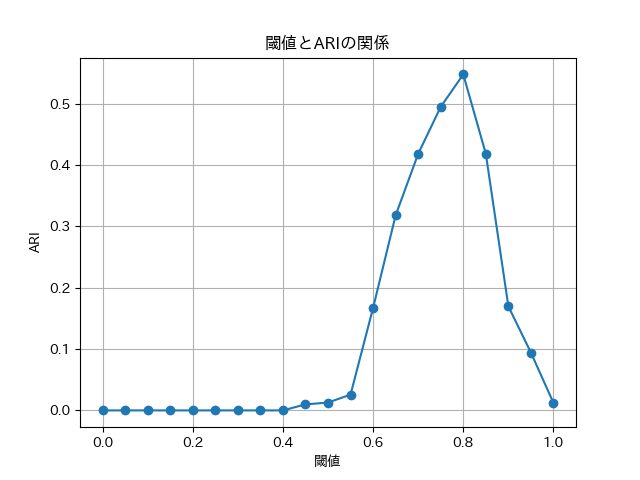
\includegraphics[scale=0.8]
    {contents/images/cw_graph.png}
  \caption{閾値ごとのARIの結果\label{fig:cw_graph}}
\end{figure}

\noindent
図\ref{fig:cw_graph}より, 閾値を0.8としたときのARIが最も高くなることがわかった. したがって本研究では全てのデータのクラスタリングにおいて閾値は0.8に設定して行った. 

\subsection{他の手法との比較}
本研究で実装したChinese Whispersと, 一般的に使用されているクラスタリングであるK-Means, 階層型クラスタリングを比較することにより本研究のクラスタリング手法の性能を検証する. 

K-Meansは非階層型クラスタリングのアルゴリズムである. まず, 互いのデータをランダムなクラスターに配置したのちにクラスターごとの重心を計算する. そして, 各データに対して重心が最も近いクラスターを割り振り重心を再計算する. このステップを重心が動かなくなるまで繰り返すことによりクラスターを決定する.

階層型クラスタリングはデータからクラスターの階層構造を抽出する手法である. 最初は各データがそれぞれ1つのクラスターを持つ. そしてクラスター間の距離が最も近い2つのクラスターを1つのクラスターにまとめる. これを繰り返していき, クラスターを大きくしていく. クラスター間距離の計算方法はウォード法や群平均法, 最短距離法, 最長距離法などいくつかの方法がある. 

K-Means, 階層型クラスタリングは共にクラスター数を事前に選択する必要があるためクラスター数をいくつに設定すると最もARIが高くなるか検証した. 
K-Meansにおけるクラスター数とARIの関係を図\ref{fig:kmeans_graph}, 階層型クラスタリングにおけるクラスター数とARIの関係を図\ref{fig:agg_graph}にそれぞれ示す.

\begin{figure}[H]
  \centering
  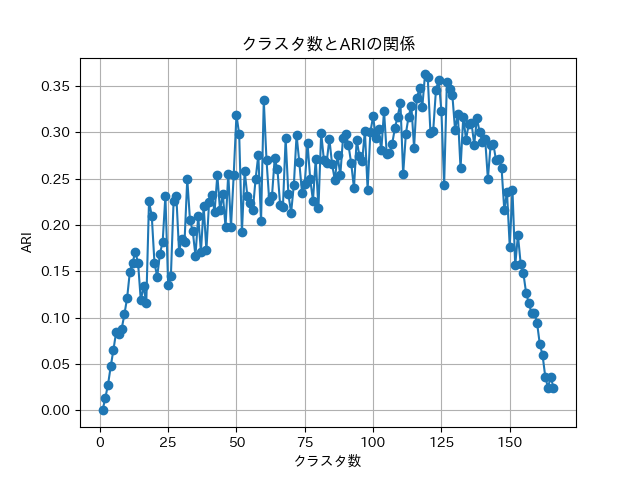
\includegraphics[scale=0.8]
    {contents/images/kmeans_graph.png}
  \caption{K-Meansにおけるクラスター数ごとのARIの結果\label{fig:kmeans_graph}}
\end{figure}

\begin{figure}[H]
  \centering
  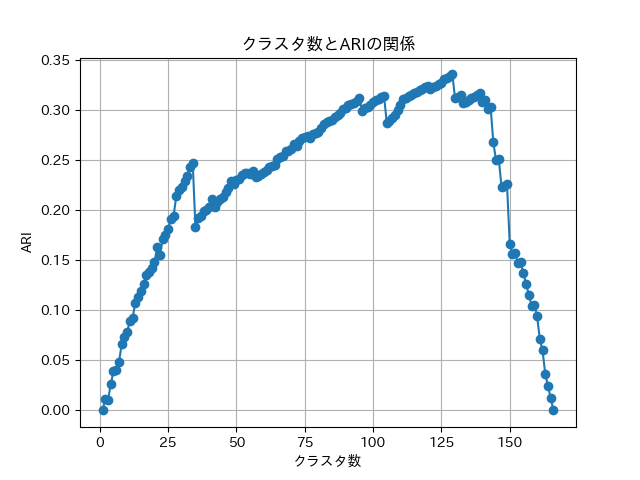
\includegraphics[scale=0.8]
    {contents/images/agg_graph.png}
  \caption{階層型クラスタリングにおけるクラスター数ごとのARIの結果\label{fig:agg_graph}}
\end{figure}

検証した結果, K-Meansではクラスター数が119, 階層型クラスタリングではクラスター数が129の時にそれぞれARIは最も高い値を示した. 次にK-Means, 階層型クラスタリングとChinese WhispersのARIの最大値を比較した結果が表\ref{tb:two_ari}である. 

\begin{table}[H]
  \caption{3つの手法におけるARI}
  \label{tb:two_ari}
  \begin{center}
  \begin{tabularx}{\linewidth}{X|r|r}
    \hline
    手法&ARIの最大値&クラスター数\\\hline\hline
    手動&-&123\\\hline
    階層型クラスタリング&0.34&129\\\hline
    K-Means&0.36&119\\\hline
    Chinese Whispers&\textbf{0.55}&144\\\hline
  \end{tabularx}\end{center}
\end{table}

比較した結果, Chinese WhispersのARIの最大値は 階層型クラスタリングよりも0.21, K-Meansよりも0.18ほど高いことが示された. 

\subsection{総括}
Chinese Whispersで作成されるグラフの閾値について検証した結果, 閾値を0.8としたときに最もARIが高い値を示すことがわかった. 
また, K-Means, 階層型クラスタリング, Chinese Whispersの3つの手法におけるARIの最大値を比較した結果, Chinese Whispersが最もARIが高くなったことから本研究のクラスタリング性能の高さを示すことができた. 

%ーーーーーーーーーーーーーーーーーーーーーーーーーーーー

\section{RQ3:可視化ツールの有用性はどうか}
\subsection{概要}
抽出, クラスタリングによって得られた結果を表示する可視化ツールの有用性について示す. 一般的にレビューの閲覧や確認で使用されるGoogle Playストアのレビュー欄と比較して, 本研究で作成した可視化ツールがレビューの分析にどのように役立つのかを記述する. 

\subsection{Google Playストアのレビュー欄}
Google Playストアのレビュー欄は図\ref{fig:google_play}, 図\ref{fig:google_play_graph}のような構成となっている. 

\begin{figure}[H]
  \centering
  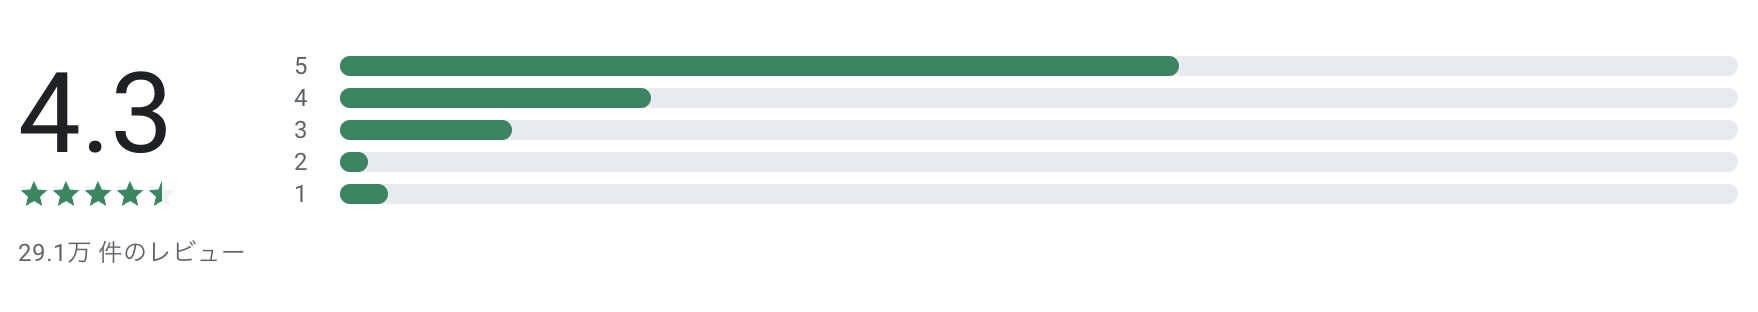
\includegraphics[scale=0.4]
    {contents/images/google_play_graph.png}
  \caption{各評価の数を表すグラフ\label{fig:google_play_graph}}
\end{figure}

\begin{figure}[H]
  \centering
  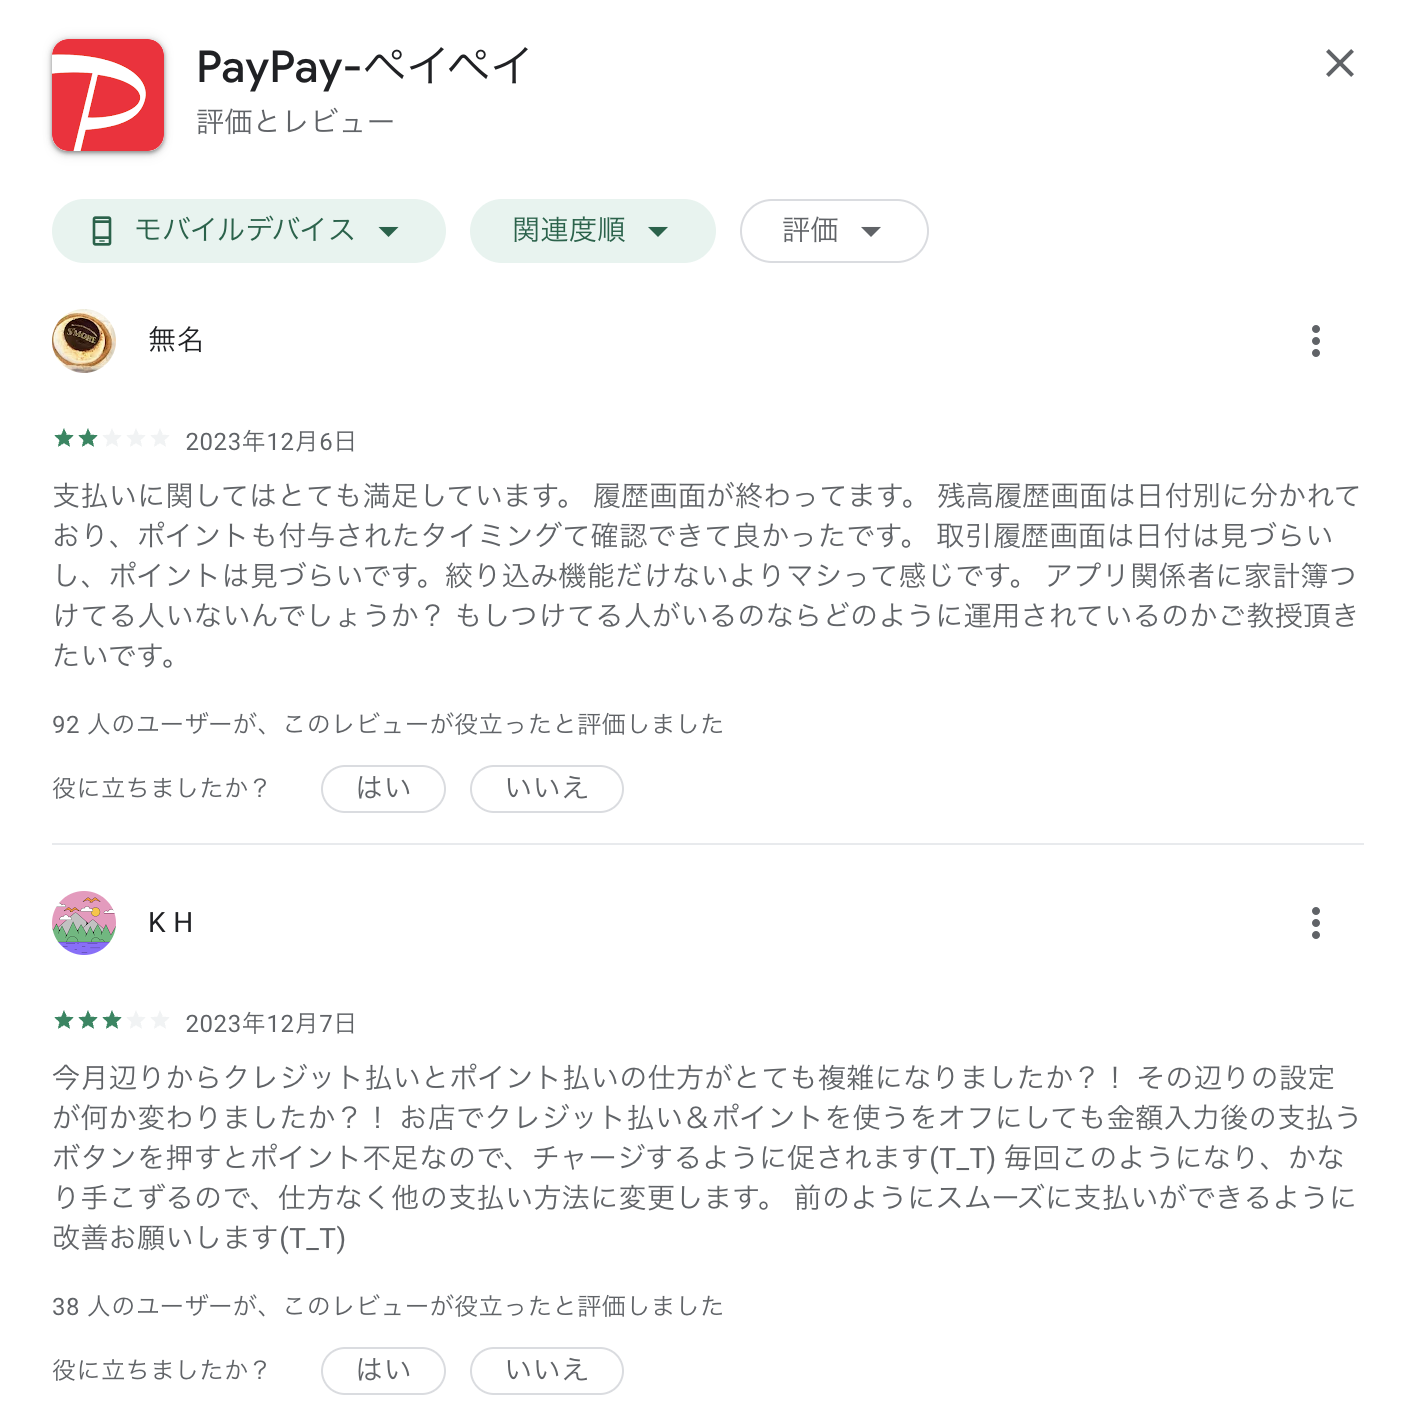
\includegraphics[scale=0.4]
    {contents/images/google_play.png}
  \caption{Google Playストアのレビュー欄\label{fig:google_play}}
\end{figure}

Google Playストアのレビュー欄では評価 (星1〜星5) がそれぞれいくつ付けられているのかを表示するグラフ (図\ref{fig:google_play_graph}) と, 各レビューが記載されている (図\ref{fig:google_play}) . 各レビューには何人のユーザが役に立ったかが記載されており, これによりユーザから見た各レビューの評価がわかる. 
また, 主な機能として評価ごとの絞り込み, 評価や時系列による並び替えがある. 

Google Playストアのレビュー欄と本研究のwebアプリの違いを示すことで本研究のwebアプリの有用性を示す. 

\subsection{キーワードと期間の検索}
このwebアプリではキーワードの検索により特定の機能に関するレビューを絞り込むことができる. また, 期間を絞り込むことにより特定の期間に投稿されたレビューのみを表示することができる.  

この機能は特にアプリのアップデート時に活用できる. アプリのアップデート時に開発者は改善した機能や新しく追加した機能が正常に動いているかどうか, アップデートの前後でレビュー数に変化があるかどうかを確認したい. そのため, この検索機能を用いて分析対象となるレビューを期間とキーワードで絞り込むことで確認するレビュー数を大幅に減らすことができる. 

図\ref{fig:paypay_search}は期間 (2021/10/21〜2021/11/11) ・キーワード (ログイン) で検索した例である. このように, 検索機能を活用して特定の期間や機能に関するレビューのみを表示することが可能となっている. 
\begin{figure}[H]
  \centering
  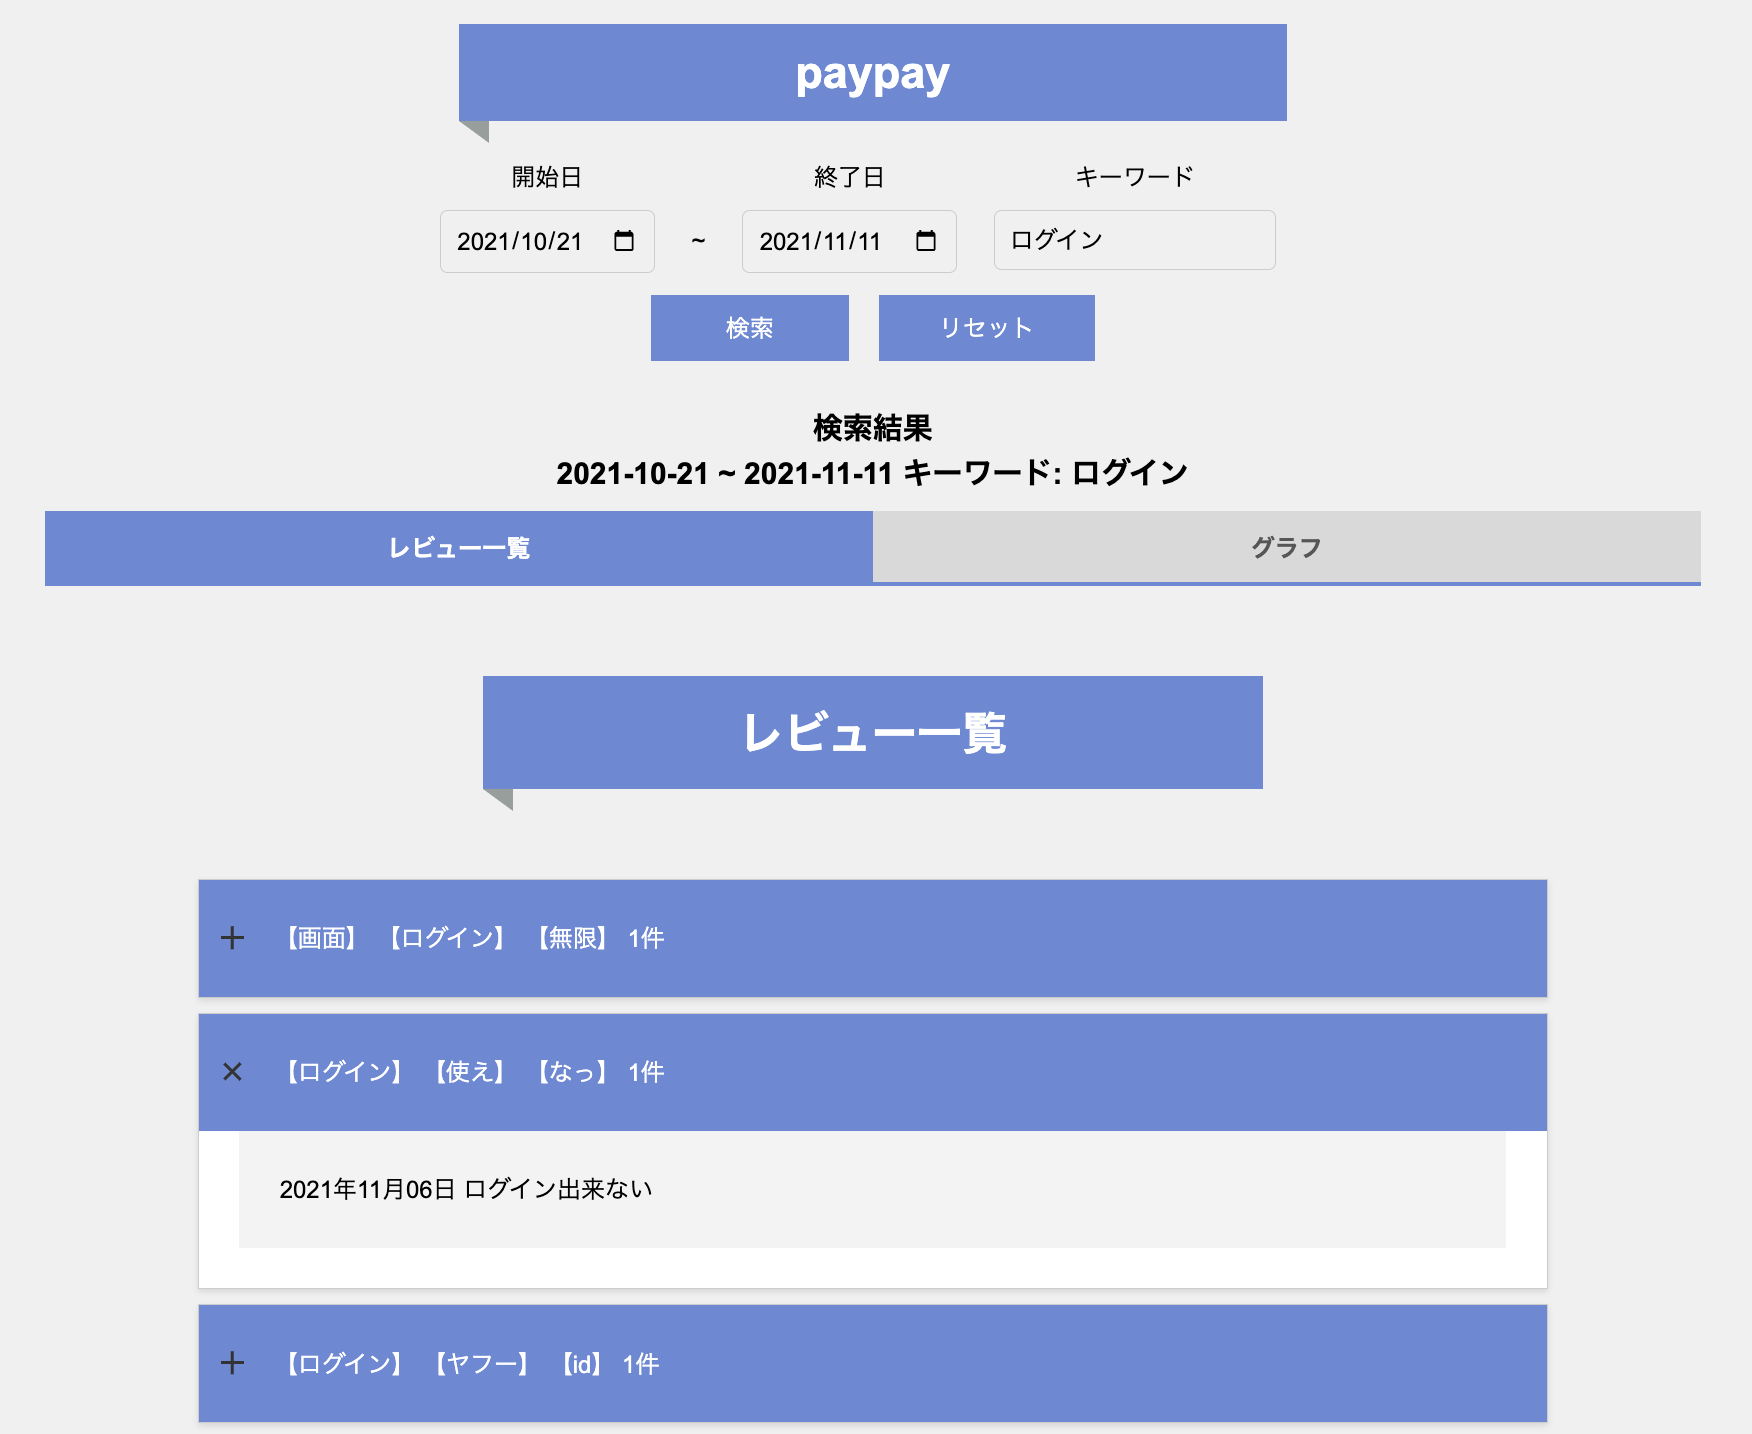
\includegraphics[scale=0.3]
    {contents/images/paypay_search.png}
  \caption{paypayのレビュー検索結果\label{fig:paypay_search}}
\end{figure}

% \subsection{アプリ間のレビュー比較}
% この可視化ツールでは一覧画面にてアプリごとのレビュー数の推移を表示することができる. そのためアプリ間でレビュー数にどのような変化があるのかを1つのグラフで確認することができる. 

% Google Playストアにおける日付とレビュー数の関係を表した折れ線グラフが図\ref{fig:google_graph}である. このグラフは右側にあるアプリ名をタップすることによりグラフ表示のON/OFFが切り替えられるようになっている. 
% また, 検索結果に応じて日付やレビュー数が動的に変更されるようになっている. 

% \begin{figure}[H]
%   \centering
%   \includegraphics[scale=0.3]
%     {contents/images/google_graph.png}
%   \caption{Google Playストアにおける日付とレビュー数の関係\label{fig:google_graph}}
% \end{figure}

% この機能を用いて, 類似した機能を持つアプリがどのような問題を抱えているかを分析することができる. 類似したアプリで見つけられた欠陥は自身の開発しているアプリで同じような欠陥が見つかる可能性がある. 
% したがって開発者はこの可視化ツールで他のアプリのレビューを確認することにより自身の開発に活用することができる. 

\subsection{レビューの分析時間短縮}
Google Playストアのレビュー欄の欠点は開発に役立たないレビューが多く存在し, 似たような機能の記述がまとまっていないため開発者が分析するのに時間がかかることである. 
このような欠点を解消したのが本研究の可視化ツールである. この可視化ツールは開発に役立つレビューかどうかをフィルタリングして類似したレビューをまとめて表示している. そのため開発者はレビューを分析する時間を短縮できる. 
また, Google Playストアのレビュー欄ではどの期間に多くのレビューが投稿されたかを確認するのに時間がかかる. しかし, 本研究の可視化ツールであれば, 日ごとのレビュー数の推移をグラフにより表示しているため, どの期間に多くのレビューが書かれているかを確認できる. 
このように本研究の可視化ツールを使用することにより, レビューの分析や閲覧にかかる時間を大幅に短縮することが可能となる. 

\subsection{多大な情報量}
本研究の可視化ツールにはGoogle Playストアのレビューだけではなく, Twitterのツイートも表示している. そのためユーザのさまざまな意見を閲覧することができる. 
2021年10月21日から2021年12月15日に取得されたGoogle Playストアのレビュー7,912件とTwitterのツイート1,525,211件のうち, 抽出モデルによって抽出されたキーフレーズの数は表\ref{tb:app_count}となった. 

\begin{table}[H]
  \small
  \caption{抽出されたキーフレーズの数}
  \label{tb:app_count}
  \begin{center}
  \begin{tabularx}{\linewidth}{X|r|r}
    \hline
    アプリ名&Google Playストア&Twitter\\\hline\hline
    にゃんトーク&\textbf{199}&144\\\hline
    スマートニュース&\textbf{615}&134\\\hline
    PayPay&546&\textbf{10,706}\\\hline
    Coke ON&\textbf{1,212}&568\\\hline
    Google Fit&\textbf{570}&307\\\hline
    Simeji&359&\textbf{1,441}\\\hline
    Lemon8&25&\textbf{27}\\\hline
    楽天ペイ&541&\textbf{1,253}\\\hline
    majica&\textbf{1,084}&85\\\hline
    LINE MUSIC&519&\textbf{2,694}\\\hline
    BuzzVideo&146&\textbf{299}\\\hline
    ファミペイ&163&\textbf{314}\\\hline
    CapCut&166&\textbf{261}\\\hline\hline
    合計&6,145&\textbf{18,233}\\\hline
  \end{tabularx}\end{center}
\end{table}

\noindent
表\ref{tb:app_count}からわかるように同一期間で比較した場合, Google PlayストアよりもTwitterの方が抽出されたキーフレーズの数が多いことがわかる. 
この結果からTwitterのツイートを分析対象として含むことは有用であることがわかる. 

\subsection{総括}
本研究で作成された可視化ツールを使用することにより, 開発者がレビューを確認する時間の短縮や効率の向上につながっている. また, Twitterのツイートを分析対象としていることにより提供できる情報量が多いことはこの可視化ツールの大きな特徴である. レビュー分析を効率化させることは開発者にとって1つの課題であるため本研究の可視化ツールは非常に有用であると考えられる. 

\section{妥当性の脅威}
\subsection{対象アプリ}
本研究の対象アプリはデータ取得の問題により先行研究のアプリに合わせている. アプリの選択はカテゴリーについて考慮されていないためそれぞれのカテゴリーにおける提案手法の有効性は確保されていない. 
したがって, 様々なカテゴリーに属する多くのアプリのレビューデータに提案手法を実行して, 有効性を確認する必要がある. 

\subsection{トレーニングデータ}
本研究では情報工学科の学生2人により10,000件のレビューからトレーニングデータを作成した. RQ1でも述べたように, このトレーニングデータの精度には改善の余地がある. 
トレーニングデータの精度を向上させるために, アプリの開発者などレビューに関する専門的知識を持つ人がトレーニングデータを作成する, トレーニングデータを作成する人数を増やして議論するなど工夫が必要である. 
また, 本研究ではトレーニングデータの数を増やすことにより精度が上がるかどうかを検証していない. そのため, データ数と自動抽出精度の関係性に関して更なる調査が必要である. 

\subsection{自動抽出とクラスタリングの関係性}
提案手法では自動抽出したキーフレーズを意味に応じてクラスタリングしている. したがって, クラスタリングの精度は自動抽出の精度に依存する. 
RQ1の結果から自動抽出には改善の余地が見られるため, クラスタリングした際に精度の悪さが蓄積する危険性がある. クラスタリングの精度向上には自動抽出の精度向上が必要であると考えられる. 
\chapter{結論}
\label{chap:keturon}

レビューの中にある問題のある機能やアプリに対する要望に関する報告を自動抽出してからその抽出した情報を元に分類することにより分類精度を向上させつつ, 粒度の高い分類を行う. また, その結果を時系列やアプリごとにWebブラウザ上に出力し, 開発者を支援する可視化ツールを提案した.

3つのRQにて自動抽出, 分類の性能を評価し, 可視化の有用性を示すことができた. 
%%%%%%%%%%%%%%%%%%%%%%%%%%%%%%%%%%%%%%%%%%%%%%%%%%%%%%%%%%%%%%%%%%
% 論文本体おわり                                                 %
%%%%%%%%%%%%%%%%%%%%%%%%%%%%%%%%%%%%%%%%%%%%%%%%%%%%%%%%%%%%%%%%%%

%%%%%%%%%%%%%%%%%%%%%%%%%%%%%%%%%%%%%%%%%%%%%%%%%%%%%%%%%%%%%%%%%%
% 謝辞. 感謝の気持ちを書く. \acknowledge以下に直接書くか,        %
%   \input で\acknowledge を記述したファイルを読み込む           %
%%%%%%%%%%%%%%%%%%%%%%%%%%%%%%%%%%%%%%%%%%%%%%%%%%%%%%%%%%%%%%%%%%
\acknowledge


本研究を行うにあたり, 日頃から親身にご指導をしていただいた慶應義塾大学理工学部情報工学科の高田眞吾教授に感謝いたします.
そして, 未熟な私を様々な面で身近で支えていただいた慶應義塾大学理工学部情報工学科 高田研究室の先輩方, 同期の皆様に心から感謝いたします. 


2024年1月 
\begin{flushright}
  {\Large 佐藤 響}
\end{flushright}
%%%%%%%%%%%%%%%%%%%%%%%%%%%%%%%%%%%%%%%%%%%%%%%%%%%%%%%%%%%%%%%%%%
% 謝辞おわり                                                     %
%%%%%%%%%%%%%%%%%%%%%%%%%%%%%%%%%%%%%%%%%%%%%%%%%%%%%%%%%%%%%%%%%%

%%%%%%%%%%%%%%%%%%%%%%%%%%%%%%%%%%%%%%%%%%%%%%%%%%%%%%%%%%%%%%%%%%
% 参考文献                                                       %
% \bibliographystyle に選択した参考文献表示方法を入れる          %
% 参考文献内容は, bibtexで管理するのが楽. thesis.bibに書こう.    %
%%%%%%%%%%%%%%%%%%%%%%%%%%%%%%%%%%%%%%%%%%%%%%%%%%%%%%%%%%%%%%%%%%
\bibliographystyle{jplain}
\bibliography{thesis}
%%%%%%%%%%%%%%%%%%%%%%%%%%%%%%%%%%%%%%%%%%%%%%%%%%%%%%%%%%%%%%%%%%
% 参考文献おわり                                                 %
%%%%%%%%%%%%%%%%%%%%%%%%%%%%%%%%%%%%%%%%%%%%%%%%%%%%%%%%%%%%%%%%%%

% \appendix



\end{document}

